\documentclass[11pt,preprint, authoryear]{article}

\pagestyle{plain}

\usepackage{lmodern}

% LANDSCAPE package
\usepackage{pdflscape}

% MATH packages
\usepackage{amssymb,amsmath} %amsthm, amsfonts}

% SPACING passed through from .Rmd doc
\usepackage{setspace}
\setstretch{1.5}

% Wrap around which gives all figures included the [H] command, or places it "here". This can be tedious to code in Rmarkdown.
\usepackage{float}
\let\origfigure\figure
\let\endorigfigure\endfigure
\renewenvironment{figure}[1][2] {
    \expandafter\origfigure\expandafter[H]
} {
    \endorigfigure
}

\let\origtable\table
\let\endorigtable\endtable
\renewenvironment{table}[1][2] {
    \expandafter\origtable\expandafter[H]
} {
    \endorigtable
}

\DeclareMathSizes{24}{26}{22}{22}

\usepackage[round]{natbib}
\bibliographystyle{natbib}
\def\bibsection{\section*{References}} %%% Make "References" appear before bibliography

% package for nice tables
\usepackage{longtable}

% package for ruling lines in tables e.g. midrule
\usepackage{booktabs}

% set margins
\usepackage[left=3.5cm, right=2cm, top=30mm ,bottom=2cm, includefoot]{geometry}
\usepackage{fancyhdr}
\usepackage[bottom, hang, flushmargin]{footmisc}
\usepackage{graphicx,grffile}
%\numberwithin{equation}{section} % commented out because it messes up equation numbering
%\numberwithin{figure}{section} % commented out because it messes up figure numbering
%\numberwithin{table}{section} % commented out because it messes up table numbering
\setlength{\parindent}{0cm}
\setlength{\parskip}{1.3ex plus 0.5ex minus 0.3ex}
\usepackage{textcomp}
\renewcommand{\headrulewidth}{0pt}

% HERE we try to create a custom table column
\usepackage{array}
\newcolumntype{x}[1]{>{\centering\arraybackslash\hspace{0pt}}p{#1}}

% CHANGE this to change how hyperlinks appear in text
\usepackage{hyperref}
\hypersetup{breaklinks=true,
            bookmarks=true,
            colorlinks=true,
            citecolor=black,
            urlcolor=black, % CHANGE this to make url links coloured
            linkcolor=black, % CHANGE this to make section links coloured
            pdfborder={0 0 0}}
						
\urlstyle{same}  % don't use monospace font for urls


\setlength{\parindent}{0pt}
\setlength{\parskip}{6pt plus 2pt minus 1pt}

\setlength{\emergencystretch}{3em}  % prevent overfull lines

% STILL haven't figured tightlist out
\providecommand{\tightlist}{%
  \setlength{\itemsep}{0pt}\setlength{\parskip}{0pt}}

\setcounter{secnumdepth}{5}

% Use protect on footnotes to avoid problems with footnotes in titles
\let\rmarkdownfootnote\footnote%
\def\footnote{\protect\rmarkdownfootnote}
\IfFileExists{upquote.sty}{\usepackage{upquote}}{}

% pass through extra packages specified by user
\usepackage{bm}

%%%%%%%%%%%%%%%%%%%%%%%%%%%%%%%%%%%%%%%%%%%
%%%%%%%%%%%%%%%%%% EDIT TITLE %%%%%%%%%%%%%%%%%%
%%%%%%%%%%%%%%%%%%%%%%%%%%%%%%%%%%%%%%%%%%%

% change title format to be more compact
\usepackage{titling}

% create subtitle command for use in maketitle
\newcommand{\subtitle}[1]{
  \postauthor{
    \begin{center}\large#1\end{center}
    }
}

\setlength{\droptitle}{-1em}
\pretitle{\vspace{\droptitle}\centering\Huge}
\posttitle{\par\vskip 5.5em}

\title{
{\scshape\Large Department of Statistics 2019}\\
{\vskip 2.5em \scshape Predicting Community Engagement with Questions in the StackOverflow
Online Question-Answer Community}\\
%{\includegraphics{lse.png}} % if you want to include LSE logo
}

\preauthor{\centering\LARGE}
\postauthor{\par\vskip 4em}

\author{Candidate Number: 10140}
\subtitle{\vspace{4em} Submitted for the Master of Science, London School of Economics,
University of London} % comment this out and you get *Missing \begin{document}*

\predate{\centering\Large}
\postdate{\par}

\date{\scshape August 2019}

\usepackage{color}

\usepackage[usenames,dvipsnames,svgnames,table]{xcolor}

\usepackage{tocloft}

%%%%%%%%%%%%%%%%%%%%%%%%%%%%%%%%%%%%%%%%%%%
%%%%%%%%%%%%%%%% BEGIN DOCUMENT %%%%%%%%%%%%%%%%
%%%%%%%%%%%%%%%%%%%%%%%%%%%%%%%%%%%%%%%%%%%

\begin{document}

% Header and Footers
\pagestyle{fancy}
\chead{}
\rhead{}
\lfoot{}
\rfoot{} 
\lhead{}
%\rfoot{\footnotesize Page \thepage\ } % "e.g. Page 2"
\cfoot{\footnotesize \thepage\\}

% i, ii, iii etc. page numbering
\pagenumbering{roman}

\maketitle

\thispagestyle{empty}

\clearpage

\setcounter{page}{1}

% table of contents, list of figures and tables
\renewcommand{\contentsname}{Table of Contents}
\tableofcontents
\newpage
\listoffigures
\newpage
\listoftables
\newpage

% ACKNOWLEDGEMENTS SECTION
\begin{center}
\section*{Acknowledgement}
\end{center}
I would like to dedicate this work to my wife Bronwyn. Words cannot describe how much I appreciate your unending love, support and patience over this past year that we have spent together in London.

\clearpage

% SUMMARY SECTION
\section*{Summary}

Formulating constructive questions and receiving answers to these
questions is crucial to how we examine, learn from and critically
analyse the world around us. The evolution of the world wide web and the
technologies that have emerged with it have given us an unprecedented
ability to engage with and learn from individuals around the globe.
While substantial attention has been dedicated to finding the right
answers (just ask Google), comparatively less has been devoted to how we
can improve the constructiveness of our questions. The domain of online
question-answer (Q\&A) communities is one setting where relevant and
well-researched questions are of particular importance, not least
because expert resources are scarce in contrast to question volumes. One
way to address this problem of ``information overload'' is to provide
questioners with accurate predictions of their question
constructiveness, prompting revision of questions before demand is added
on expert resources. In light of this goal, this paper builds on
predictive modelling and question quality research in online Q\&A
communities in three ways: 1) I predict community engagement, which I
consider a more objective and definitive response than question quality,
2) I accept each questions' community-granted ``score'' as an
informative and comprehensive measurement of community engagement, and
3) I predict a range of community engagement rather than discrete
categories. Using only textual question content available when questions
are initially submitted, I analyse monthly datasets from the largest
online computer programming Q\&A community,
\href{https://stackoverflow.com/}{StackOverflow.com}. Contrary to recent
research, I find that features derived question content lead to
negligible model performance improvement over a low baseline across
datasets. While this work shows that accurate prediction of online Q\&A
community engagement is still an ambitious goal, it serves as a stepping
stone in addressing information overload in these platforms and
improving their functioning substantially.

\clearpage

% 1, 2, 3 etc. page numbering
\pagenumbering{arabic}

\newpage

\section{\texorpdfstring{Introduction
\label{Intro}}{Introduction }}\label{introduction}

Modern interpersonal communication technologies made possible by the
internet have afforded us an exceptional level of connection and
engagement with the world. Billions of individuals now interact online
instantly, not only with people that they know, but with strangers
thousands of miles away. One avenue of online interaction that has
become an extremely popular way in which users share knowledge about
diverse and nuanced subject matter is question-and-answer (Q\&A)
websites such as Yahoo! Answers, Quora, the StackExchange family and
forums of Massive Online Open Courses (MOOCs). These websites serve as
dynamic, engaging platforms where users seek answers to and discussions
on complex, technical questions that modern search engines are evidently
yet unable to fully address.

Producing relevant, well-researched and high-quality questions in online
Q\&A fora is especially valuable, not least since these platforms suffer
in particular from a low ratio of expert resources to volume of new
questions - an example of an increasingly ubiquitous problem known as
\emph{information overload}, of which a broader summary can be found in
Eppler and Mengis (2004). The overarching hypothesis of this research is
that information overload in online Q\&A communities would be mitigated
if questioners were notified in advance of how well their questions
would be received by a community. This would allow them to iterate and
increase the ``signal'' of their questions before exerting demand on
community resources. If this were possible, it would not only benefit
questioners as they would more effectively garner expert answers to
their improved questions, but also entire communities as overall
functioning and efficiency is enhanced community-wide.

Predicting the extent to which online communities would react positively
to user questions in real time is a non-trivial problem however, since
predictions must be made using only the information available when new
questions are formulated. This implies that predictive models must learn
from features derived from question content alone and not features such
user characteristics, final webpage viewing statistics and so on.
Ideally, final predictions given to questioners would also be highly
granular and direct questioners towards how best to improve their
questions as a type of recommendation system, however the aim of this
research is only to take one step forward from previous work on
questions in online Q\&A communities and ascertain if community
engagement in online Q\&A fora can actually be predicted with some
measure of accuracy.

The broad research question for this paper can therefore be summarised
as the following:

\begin{center}
\emph{To what extent can community engagement with questions in online Q\&A communities be accurately predicted using only question content?}
\end{center}

While there is a substantial amount of literature that has addressed
online Q\&A communities, curiously the focus has been on identifying
expert users and high quality answers rather than on questions, despite
questions being the entry point for every interaction in communities. In
an attempt to answer the research question above, I build on the small
collection of research on \emph{question quality} in online Q\&A fora
and draw heavily on work done by Ravi \emph{et al.} (2014) with data
from the popular computer programming community
\href{https://StackOverflow.com}{StackOverflow}.

Ravi \emph{et al.} (2014) predicted a binary notion of question quality
(``good'' versus ``bad''), and their classifier significantly beats out
a strong baseline with accuracies of 55.5\%, 65.8\% and 64.2\% for a
length, textual-content and latent Dirichlet allocation (LDA) latent
topic model respectively. I critique, mirror and expand the analysis of
Ravi \emph{et al.} (2014) in three core ways: 1) I consider community
engagement to be a more objective and definitive metric to predict on
than question quality, 2) I use the community-granted question
\texttt{Score} as a comprehensive measurement of community engagement,
and 3) I employ a regression model to allow for predictions to be
continuous and informative as opposed to binary.

The \texttt{Score} variable is an aggregation of all community
\emph{up-votes} and \emph{down-votes} for each question in the
StackOverflow community, and I predict this variable in multiple monthly
StackOverflow datasets using only the textual content of questions. In
line with the analysis of Ravi \emph{et al.} (2014), I engineer length,
textual-content and latent topical features from question content for
the prediction problem. I use regularised regression for the learning
task and evaluate models using root-mean-square error (RMSE).

It should be noted that the goal of this research is quantitative
prediction rather than qualitative, causal or inferential analysis. I
leave it to further research to address more precisely the \emph{how}
and \emph{why} of community engagement in online Q\&A communities,
rather than just the \emph{if} that is explored here. To my knowledge
this research is the first of its kind to test latent topic models on a
continuous, objective measurement of online community engagement as well
as pertain to a feasible and valuable use-case, which I believe makes it
a practical and unique contribution.

The findings from my analysis show that there is still much work to be
done to accurately predict community engagement in online Q\&A fora.
Contrary to the impressive classification accuracies in the results of
Ravi \emph{et al.} (2014), I find that models which include textual
question content features do not perform any better over a modest
baseline of constant mean prediction. Evidently, accurately predicting a
continuous measurement of community engagement in a regression setting
is an ambitious task, and I recommend that future research employ more
sophisticated models and feature engineering, as well as incorporate
time-series aspects.

In the following section I discuss the relevant literature in more
detail. This is followed by section \ref{Method} which discusses the
data, explores and validates my choice of the \texttt{Score} variable as
an objective measurement of community engagement, and describes the
predictive model used. Section \ref{Results} presents and discusses the
results, section \ref{Recom} explores some recommendations for further
research and finally section \ref{Concl} concludes.

\newpage

\section{\texorpdfstring{Literature Review
\label{Lit}}{Literature Review }}\label{literature-review}

My work involves the extraction of textual features from question
content submitted to the online Q\&A fora, and the training and
evaluation of predictive regression models. This section provides brief
summaries of previous work related to this research problem. Section
\ref{qacomm} discusses previous work on online Q\&A communities and
section \ref{qquality} discusses work on predicting \emph{question
quality} in online Q\&A communities. Section \label{ravi} summarises the
approach and results of Ravi \emph{et al.} (2014), and finally section
\label{lda_lit} briefly introduces how latent topic models have been
applied to questions in online Q\&A fora.

\subsection{\texorpdfstring{Question-Answer Communities
\label{qacomm}}{Question-Answer Communities }}\label{question-answer-communities}

There is a substantial collection of research that has investigated
online Q\&A communities. Prior work has addressed answer quality (Jeon
\emph{et al.}, 2006; Shah and Pomerantz, 2010; Tian \emph{et al.},
2013), satisfaction of questioners (Liu \emph{et al.}, 2008) and the
behaviour of highly productive, expert community members (Riahi \emph{et
al.}, 2012; Sung \emph{et al.}, 2013). Two common frameworks for prior
work have been the optimisation of routing questions to experts (Li and
King, 2010; Li \emph{et al.}, 2011; Zhou \emph{et al.}, 2012; Shah
\emph{et al.}, 2018), and matching questions in accordance with answerer
interest in the form of a recommendation system (Wu \emph{et al.}, 2008;
Qu \emph{et al.}, 2009; Szpektor \emph{et al.}, 2013).

My research differs from this previous work on Q\&A fora in two
respects. Firstly, I focus on questions rather than user or answer
characteristics, not only because they have received substantially less
attention in the literature, but because it has been shown that question
quality can substantially impact the quality of answers (Agichtein
\emph{et al.}, 2008). Questions in online Q\&A fora are also the initial
touch point from which all community engagement follows - maximising
positive community engagement with questions will thus almost certainly
improve the functioning of these communities.

I also deviate from prior research in the framework that I place this
research in. I steer clear of the systems-based optimisation of
question-answer routing/matching and instead concentrate on how
questioners can be nudged to improve the content of their questions
before adding demand to community resources. Although there is
substantial literature on community engagement in a broad range of
fields and disciplines, this literature is either too disparate from the
field of research in this paper or focuses on online engagement in other
forms. To my knowledge therefore, this work is the first of its kind to
characterise and predict community engagement with questions in the
context of online Q\&A fora. Owing to the fact that the framework I have
chosen coincides with a large collection of research on predicting
question quality in online Q\&A communities, I discuss this literature
next.

\subsection{\texorpdfstring{Question Quality
\label{qquality}}{Question Quality }}\label{question-quality}

Naturally, community engagement and question quality go hand in hand:
high quality questions will no doubt lead to positive community feedback
in the form of numerous up-votes, answers and discussion promoting
comments. I argue in the following section that \emph{community
engagement} is a more accurate and thorough definition of what the
following literature claims to measure, but for the sake of discussion I
will refer to question quality here as well.

A recent line of work has looked at predicting question quality in the
large Q\&A community \href{http://answers.yahoo.com}{Yahoo! Answers}
(Agichtein \emph{et al.}, 2008; Bian \emph{et al.}, 2009; Li \emph{et
al.}, 2012) - a dataset which has metrics for assessing answer quality
in the form of answer up-votes, but regrettably lacks a similarly
community-attributed and objective metric for question quality. This has
resulted in subjective attempts at defining question quality: Agichtein
\emph{et al.} (2008) define question quality using questions' semantic
features (lexical complexity, punctuation, typos etc.), Bian \emph{et
al.} (2009) use manual labels for 250 questions and a semi-supervised
coupled mutual reinforcement framework to label a larger number of
questions, and Li \emph{et al.} (2012) combine the number of answers,
number of tags, time until first answer, author judgement and domain
expertise to construct their ground truth.

Fortunately, I analyse data from the
\href{https://StackOverflow.com}{StackOverflow} Q\&A community which is
rich in objective community-attributed metrics such as question up- and
down-votes, comments, and views, all of which is over and above the
textual content of questions and answers themselves. These metrics are
objective in the sense that they do not require construction or
labelling form the researchers' side, and subsequently allow for large
collections of questions to be analysed automatically.

Another aspect of the literature that has evolved substantially are the
models employed to predict question quality. Previous work has modelled
question quality based on the reputation of the questioner, question
categories and lexical characteristics of questions such as length,
misspelling, words per sentence etc. (Agichtein \emph{et al.}, 2008;
Bian \emph{et al.}, 2009; Anderson \emph{et al.}, 2012; Li \emph{et
al.}, 2012). By ignoring the actual textual and topical content of
questions and focusing on features of the questioner however, these
approaches would perform poorly on questions from new users without a
community history.

Since my research goal is centred around predicting community engagement
for all community members, and in particular new and inexperienced users
who are more likely to receive negative community responses to poorly
constructed questions, I use only features available when a question is
initially asked and forego features derived from user attributes. The
methodology that I have thus far laid out mirrors work done by Ravi
\emph{et al.} (2014) to predict question quality for the StackOverflow
community. Since I will be closely emulating their methodology, I now
demonstrate their contributions.

\subsection{\texorpdfstring{Ravi \emph{et al.} (2014)
\label{ravi}}{Ravi et al. (2014) }}\label{ravi2014}

Ravi \emph{et al.} (2014) analyse a large number of questions from the
StackOverflow community to predict a binary notion (i.e. ``good'' versus
``bad'') of question quality using features derived from question
length, textual-content and latent topics. Their \emph{length} model
achieves an accuracy of 55.5\%, their \emph{text} model achieves 65.8\%
accuracy, their global \emph{topic} model achieves 64.2\% accuracy, a
combined model with all three types of features obtains 70.5\% accuracy,
all above a modest page-view feature benchmark of 61.1\%.

They compare their significant results to a baseline ``popularity''
model that only includes a variable indicating question webpage views
(which achieves 61.1\% accuracy), and subsequently claim that their
models are able to capture a notion of question quality that extends
beyond popularity. Owing to these impressive results and the appeal that
these models could be used to successfully predict community engagement,
my research closely follows their methodology, but also critiques and
extends it in a number of ways.

The first and clearest distinction in my analysis concerns the response
variable that is predicted. Ravi \emph{et al.} (2014) decide to
construct a composite response variable by dividing the
community-attributed question \texttt{Score} (the aggregation of all
user up-votes and down-votes) by the number of views a question
receives, or a questions' \texttt{ViewCount} (which is also the
independent variable that is used in their benchmark popularity model).
While they rightly state that using the \texttt{Score} variable alone
risks conflating ``question quality'' and ``popularity'' since questions
that receive higher views are more likely to receive votes, my research
objective differs in that I aim to predict community engagement rather
than question quality - I thus use only the question \texttt{Score} as
my response variable. As will be expanded upon later, I believe this
metric comprehensively characterises within-community engagement, of
which popularity and the ability to attract views is an integral
component.

Out of the 410~049 questions that Ravi \emph{et al.} (2014) extract
between 2008 and 2009, they further define the ``worst'' and ``best''
questions according to a rather arbitrary threshold of 0.001 on their
\texttt{Score}/\texttt{ViewCount} metric, resulting in only 33~199
``bad'' questions being eventually labelled and analysed. On the other
hand, my data selection consists of using all questions from five
monthly StackOverflow datasets in 2009, which coincides with the time
frame of extracted questions in Ravi \emph{et al.} (2014), but not in
dataset size. While the reasons for my choice of dataset time-span will
be more thoroughly discussed later, I believe it is good practice to
include all the questions for a given time-period owing to the aim of
providing accurate predictive information to questioners. I therefore do
not select a specific subset of questions.

The fact that I predict on the \texttt{Score} variable as a continuous
measurement of community engagement also has a number of advantages.
Firstly, any decisions on potentially arbitrary label boundaries for
discrete categories of questions are eliminated, and indeed there is
actually no need for categories of questions since each questions'
community engagement is represented on a continuous range. Providing
predictions of a questions' \texttt{Score} to questioners as an
indication of how well the StackOverflow community will react to their
question is also more informative than a binary good/bad prediction, and
has the added benefit of being easily interpreted and understandable.
Lastly, predicting on the \texttt{Score} variable alone ensures that
when I consider the benchmark \texttt{ViewCount} model, I am not
predicting on a composite variable that incorporates \texttt{ViewCount}
itself.

More broadly, I believe a framework of community engagement is more
robust and methodologically accurate than a rationale of question
quality. I am of the opinion that question quality is much more nuanced
than the prior research has asserted, not least because the definition
of quality itself is highly subjective. As an example, while most
communities may universally value certain aspects of questions such as
legibility, coherence, relevance and prior-research etc., there are
numerous question traits that communities could value to different
extents - i.e.~closed-end questions being valued in the natural sciences
as opposed to discussion-promoting questions in the social sciences.

Beyond differences in inter-community or even intra-community valuation
of questions, a community's notion of ``quality'' could also evolve over
time. A framework of community engagement therefore allows for
heterogeneity in how questions are valued across communities,
sub-communities and over time, yet it still preserves a notion of
\emph{positive} or \emph{negative} engagement in metrics that are
assumed to measure it.

Although I extend the methodology of Ravi \emph{et al.} (2014) in the
key areas discussed above, I will emulate their prediction task to
ascertain whether these models are as effective in this new framework
and in a regression setting. Since a substantial development in the
analysis of Ravi \emph{et al.} (2014) was the use of features derived
from latent topics, I briefly introduce this literature next.

\subsection{\texorpdfstring{Topic Models
\label{lda_lit}}{Topic Models }}\label{topic-models}

Bayesian inference schemes have recently become prominent in solving a
range of structured Natural Language Processing (NLP) prediction
problems owing to their ability to allow researchers to include prior
knowledge flexibly, as well as to manage uncertainty regarding model
parameters (Chiang \emph{et al.}, 2010). One notable application of
Bayesian inference is in topic modelling, which has recently been
employed in a broad range of NLP and information retrieval tasks, such
as query-focused summarisation (Daumé and Marcu, 2006), deriving
concept-attribute attachments (Reisinger and Paşca, 2009), co-reference
resolution across documents (Haghighi and Klein, 2010), computing
selection preferences (Ritter \emph{et al.}, 2010) and name ambiguity
resolution (Kozareva and Ravi, 2011).

LDA was originally introduced by David Blei and his co-authors in 2003
(Blei \emph{et al.}, 2003) and it remains a popular topic model used to
infer a set of topics inherent in a corpus (collection) of documents.
LDA is an unsupervised generative probabilistic model which assumes that
each document in a corpus is a mixture of some number of hidden topics,
and that each word in a document is generated according to one of these
topics. Finer details of LDA will be discussed in section \label{lda}.

LDA has already been applied to the StackOverflow dataset by Allamanis
and Sutton (2013), however they did not attempt to predict a measurement
of community engagement with their model. In analysing the StackOverflow
dataset, Allamanis and Sutton (2013) propose a modelling technique using
three LDA models: one over the question body as a whole, another model
on the code chunks in each question, and a last model on the question
body without noun phrases.

Ravi \emph{et al.} (2014) build on the three-tiered approach of
Allamanis and Sutton (2013) and demonstrate that inferred latent topics
are significant predictors of their measurement of question quality. The
three levels that they choose to capture topical aspects of questions
are: a global model to capture topics over each question as a whole
(coinciding with the first model in in Allamanis and Sutton (2013)), a
local topic model for sentence-level topics, and finally a Mallows model
(Fligner and Verducci, 1986) which enforces structural constraints over
sentence-level topics to capture a ``global topic structure''.

I employ only the global topic model implemented in both Allamanis and
Sutton (2013) and Ravi \emph{et al.} (2014). With the continuous
\texttt{Score} variable as my measurement of community engagement, my
goal is to ascertain if latent topic models are as effective in the
framework I have developed here, as well as if results are consistent
over multiple monthly StackOverflow datasets. I begin a thorough
discussion of the data and exploration of the \texttt{Score} variable in
the next section.

\newpage

\section{\texorpdfstring{Methodology
\label{Method}}{Methodology }}\label{methodology}

My main work comprises of three parts: data preparation, data processing
which includes feature selection, and then learning and evaluation. This
section presents the above methodologies in the order stated. The
sourcing and selection of data according to specified time ranges are
discussed in section \ref{sourcing} and \ref{selection} respectively.
Final, section \ref{comgage} motivates the \texttt{Score} variable as a
measurement of community engagement, as well as discusses the
similarities of the \texttt{ViewCount} and \texttt{Score} variable and
corresponding methodological issues.

\subsection{\texorpdfstring{Data Sourcing
\label{sourcing}}{Data Sourcing }}\label{data-sourcing}

The \href{https://stackexchange.com/sites\#traffic}{StackExchange}
family of online Q\&A fora are a diverse range of over 170 community
websites covering topics from vegetarianism to quantum computing to
bicycles. Over and above the textual content of questions, answers and
comments posted since each community's conception, rich meta-data on an
array of community interactions is publicly available in XML files
compressed in 7-Zip format at
\href{http://archive.org/download/stackexchange}{archive.org/download/stackexchange}.

At over 11 years of age with 18~million questions, 11~million users and
9.3~million site visits a day,
\href{https://stackoverflow.com}{StackOverflow} is not only the oldest
and largest StackExchange Q\&A community, but is arguably the largest
dedicated computer programming community on the internet. After
launching in July 2008 StackOverflow has averaged 2~million questions
posted each year since 2012, now encounters 6~200 new questions every
day (StackExchange.com, 2019) and is ranked the 40th most popular
website according to Alexa Internet's ranking at the time of writing
(Alexa.com, 2019).

Since the StackOverflow dataset is also publicly and freely available
for selective querying on
\href{https://cloud.google.com/bigquery}{Google Big Query}, I use this
tool to extract my variables of interest from May to September 2009 in
JSON files and then convert to
\href{https://parquet.apache.org}{Parquet} format. The following
resulting variables are of interest to my analysis:

\setstretch{0.7}

\begin{itemize}
\item
  \texttt{Score}: An aggregate variable calculated from the difference
  between registered-user granted up-votes and down-votes for a question
\item
  \texttt{ViewCount}: A counter for the number of page views a question
  receives (from both registered and non-registered users)
\item
  \texttt{Title}: The text of the question title
\item
  \texttt{Body}: The text of the question body
\item
  \texttt{CreationDate}: A datetime variable indicating when the
  question was initially posted
\end{itemize}

\setstretch{1.5}

These additional variables are briefly discussed in section \ref{Vars}
as alternatives to the \texttt{Score} variable as a response variable:

\setstretch{0.7}

\begin{itemize}
\item
  \texttt{AnswerCount}: The number of answers a question has received
\item
  \texttt{CommentCount}: The number of comments a question has received
\item
  \texttt{FavoriteCount}: The number of times registered-users have
  favourited a question
\item
  \texttt{AcceptedAnswerId}: An indication of which answer the
  question-asker has selected as accepted
\item
  \texttt{LastEditDate}: A datetime variable indicating when the post
  was last edited
\item
  \texttt{ClosedDate}: A datetime variable indicating if a question was
  closed
\end{itemize}

\setstretch{1.5}

\subsection{\texorpdfstring{Data Selection
\label{selection}}{Data Selection }}\label{data-selection}

I analyse five monthly StackOverflow question datasets from May 2009 to
September 2009. This choice broaches an aspect of the research problem
that has yet to be considered in the literature - the temporality of
online Q\&A data, and the potentially very difficult challenge of
predicting \emph{future} community engagement from \emph{past} community
engagement. Predicting future community engagement is a particularly
ambitious endeavour since there is little doubt that how questioners
formulate questions and how communities value questions are subject to
change over time. The public and open nature of the StackOverflow
community, the dynamically evolving compositions of registered-users
comprising the community, and the volatile nature of the computer
programming field would all contribute temporal elements to how
questions are formulated and received in this community.

By choosing a date range close to the start of the community and by
analysing short, monthly snapshots of the StackOverflow community, a
number of key issues relating to temporal endogeneity are addressed.
Firstly, the choice of 2009 as the year of analysis ensures that I don't
include very recent questions (i.e.~in the last few years) that have not
had enough time to garner votes and views. The use of short time-spans
also minimises the possibility of questions evolving over time and being
asked by increasingly distinct groups of individuals (questioner and
question-specific variation).

In using short time-periods I also mitigate confounding aspects
regarding the community itself evolving and changing how it values and
engages with questions (community-specific variation), or the formal
structure of the community changing (community-structure variation).
Examples of the structure of the StackOverflow community changing would
include various nudges and guides that have been implemented for users
to ask better questions. Lastly, using monthly chronological datasets
results in minimal size differences between datasets. Note that my final
underlying assumption is that there are no temporal elements or trends
in the monthly datasets I analyse - I therefore do not employ
time-series models, but treat each isolated monthly dataset as
homogeneous.

The five monthly datasets have sizes ranging from 26~026 questions in
May 2009, to 33~268 in September 2009, with 153~599 questions in total.
I process and analyse the data with PySpark, a Python API for the
open-source cluster-computing framework
\href{http://spark.apache.org}{Apache Spark}.

\subsection{\texorpdfstring{A Notion of Community Engagement
\label{comgage}}{A Notion of Community Engagement }}\label{a-notion-of-community-engagement}

\subsubsection{\texorpdfstring{Potential Candidates for Community
Engagement
\label{Vars}}{Potential Candidates for Community Engagement }}\label{potential-candidates-for-community-engagement}

Since there are a number of ways that StackOverflow members engage and
interact with each other aside from the fundamental activities of
asking/answering questions and up-/down-voting questions and answers, it
is worth considering if there are candidates more suited to capturing
community engagement and informing questioners rather than the
\texttt{Score} variable. For example, questioners are able to indicate
that an answer has explicitly answered their question, users can
``favourite'' questions and there are also further privileges for users
with enough site \emph{reputation}.

Although questions on StackOverflow are open to the general public,
posting a question in the community requires registration with an email
address and a username - once registered, users start with a
\emph{reputation} level of 1. According to the guidelines of the
StackOverflow community, reputation is a ``rough measurement of how much
the community trusts you; it is earned by convincing your peers that you
know what you're talking about'' (see
meta.stackexchange.com/questions/7237/how-does-reputation-work).

\newpage

Key reputation levels for this analysis include:

\setstretch{0.95}

\begin{itemize}
\item
  1: Users can ask questions and contribute answers
\item
  15: Users can up-vote questions and answers
\item
  15: Users can flag posts to bring them to the attention of the
  community
\item
  50: Users can comment on questions and answers
\item
  125: Users can down-vote questions and answers
\item
  2000: Users can immediately edit any question or answer
\item
  3000: Users can vote to close questions that are off-topic, unclear,
  duplicates, too-broad or too opinion-based
\end{itemize}

\setstretch{1.5}

Since the \texttt{Score} variable is the aggregation of all registered
community members' up-votes and down-votes (in accordance with their
reputation levels) it is able to register both positive (up-votes),
negative (down-votes) and neutral (abstentions) community engagement.
This metric also represents a core behaviour of the majority of the
community since users can vote regardless of their reputation level.
Providing \texttt{Score} predictions of new questions to questioners
would also be highly valuable because it provides a continuous, granular
indication of how likely that will succeed in their request for
information from the community (a high score prediction) or essentially
be rejected by the community (a low or negative score).

Some metrics are easier to eliminate as alternatives to the
\texttt{Score} variable than others. \texttt{FavouriteCount}, or the
number of times a question is favourited by registered users, has no
capacity to register negative engagement (i.e.~you cannot negatively
favourite questions) and it is also not a core functioning of the
community. \texttt{CommentCount} intuitively feels like a potentially
valuable indication of community engagement, yet comments need not be
directed at the original questioner (they could be directed at other
commenters) and without employing sentiment analysis it would be
difficult to ascertain what number of comments constitute
positive/negative community engagement.

Using \texttt{AnswerCount} as the response variable could indicate to
questioners how many answers their question is predicted to receive, but
this variable would be biased downwards for more difficult questions. An
added advantage of the \texttt{Score} variable in this regard, is that
users can still up-vote difficult questions and signify that the
community appreciates the question.

\texttt{EditCount} is another continuous variable which could indicate
community engagement in the number of edits a question receives.
Unfortunately, there is again uncertainty as to whether a high value for
this variable shows that the community has had to go through much effort
to get the question into a valuable state, or otherwise indicates that
the community deems the question useful enough to spend much energy
refining it.

This leaves two variables for consideration, \texttt{ClosedDate} and
\texttt{AcceptedAnswerId}. Indeed, using the \texttt{ClosedDate}
variable to inform questioners on whether their question is likely to be
closed would be very valuable as a measurement of community engagement.
\texttt{AcceptedAnswerId} on the other hand, would effectively indicate
whether a questioner's overarching goal has been satisfied, i.e.~whether
they indicate their request for information has been completed and
therefore be of high utility to questioners. While these variables may
be highly relevant for community engagement and valuable to questioners,
they can essentially only be represented as binary variables, over which
the \texttt{Score} variable again has an advantage.

It is thus quite clear that, out of the recorded metrics available in
the StackOverflow community data, the \texttt{Score} variable is a
comprehensive and informative measurement of community engagement. One
variable that I haven't been given any attention thus far however, is
the \texttt{ViewCount} variable. As I will motivate in the next section
though, the \texttt{Score} and \texttt{ViewCount} variables measure very
similar underlying attributes, and so I now explore both of these
variables.

\newpage

\subsubsection{\texorpdfstring{Conceptualising \texttt{Score} and
\texttt{ViewCount}
\label{scorevc_vis}}{Conceptualising Score and ViewCount }}\label{conceptualising-score-and-viewcount}

While the \texttt{Score} and \texttt{ViewCount} variables may appear to
be measuring different phenomena, in this section I contrast and compare
them to motivate that they are two sides of a similar coin. The first
evidence of this is the correlations between the both variables, shown
in table \ref{tab:corr} below. With correlations ranging from 0.71 to
0.86, it is clear that they are both highly positively correlated.

\footnotesize

\begin{longtable} {@{} cc @{}}
\caption{\textbf{Score and ViewCount Correlations}}
\label{tab:corr}\\ 
\toprule
\textbf{Dataset} & \textbf{Correlation} \\ 
\midrule
May-09 & 0.86 \\
Jun-09 & 0.85 \\
Jul-09 & 0.81 \\
Aug-09 & 0.71 \\
Sep-09 & 0.76 \\
\bottomrule
\end{longtable}\begin{center} Source: Own calculations in PySpark.\end{center}

\normalsize

Descriptive statistics for both the \texttt{Score} and
\texttt{ViewCount} variables are now displayed in tables
\ref{tab:score_desc} and \ref{tab:viewc_desc}, and density plots are
made for both variables in figures \ref{fig:score_dens} and
\ref{fig:viewc_dens}. It should be noted that that \texttt{Score}
variable for each dataset was adjusted upwards by the minimum value
across datasets to allow for a log-scaled x-axis.

\footnotesize

\begin{longtable} {@{} lccccc @{}}
\caption{\textbf{Score Variable Descriptive Statistics}}
\label{tab:score_desc}\\ 
\toprule
\textbf{Dataset} & \textbf{Count} & \textbf{Mean} & \textbf{SD} & \textbf{Min} & \textbf{Max} \\ 
\midrule
May-09 &  26\ 026 &  13.3 &   142.0 &   -7 &  19\ 640 \\
Jun-09 &  28\ 555 &  13.4 &    87.2 &   -9 &   4\ 655 \\
Jul-09 &  32\ 752 &  11.3 &    76.6 &   -8 &   6\ 145 \\
Aug-09 &  32\ 998 &   9.9 &    70.8 &  -22 &   7\ 133 \\
Sep-09 &  33\ 268 &   8.7 &    47.1 &  -10 &   2\ 809 \\
\bottomrule
\end{longtable}\begin{center} Source: Own calculations in PySpark.\end{center}

\normalsize

\footnotesize

\begin{longtable} {@{} lccccc @{}}
\caption{\textbf{ViewCount Variable Descriptive Statistics}}
\label{tab:viewc_desc}\\ 
\toprule
\textbf{Dataset} & \textbf{Count} & \textbf{Mean} & \textbf{SD} & \textbf{Min} & \textbf{Max} \\ 
\midrule
May-09 &  26\ 026 &  13\ 817 &  8\ 1233  &   26 &  7\ 906\ 137 \\
Jun-09 &  28\ 555 &  13\ 948  &  77\ 666  &   26 &  3\ 488\ 812 \\
Jul-09 &  32\ 752 &  11\ 898  &  65\ 538  &   22 &  4\ 170\ 244 \\
Aug-09 &  32\ 998 &  10\ 517  &  48\ 036  &   22 &  2\ 223\ 778 \\
Sep-09 &  33\ 268 &   9\ 555  &  39\ 505  &   23 &  2\ 009\ 096 \\
\bottomrule
\end{longtable}\begin{center} Source: Own calculations in PySpark.\end{center}

\normalsize

\footnotesize

\begin{figure}
\caption{\textbf{Score Variable Density Plot}}
\label{fig:score_dens}

\begin{center}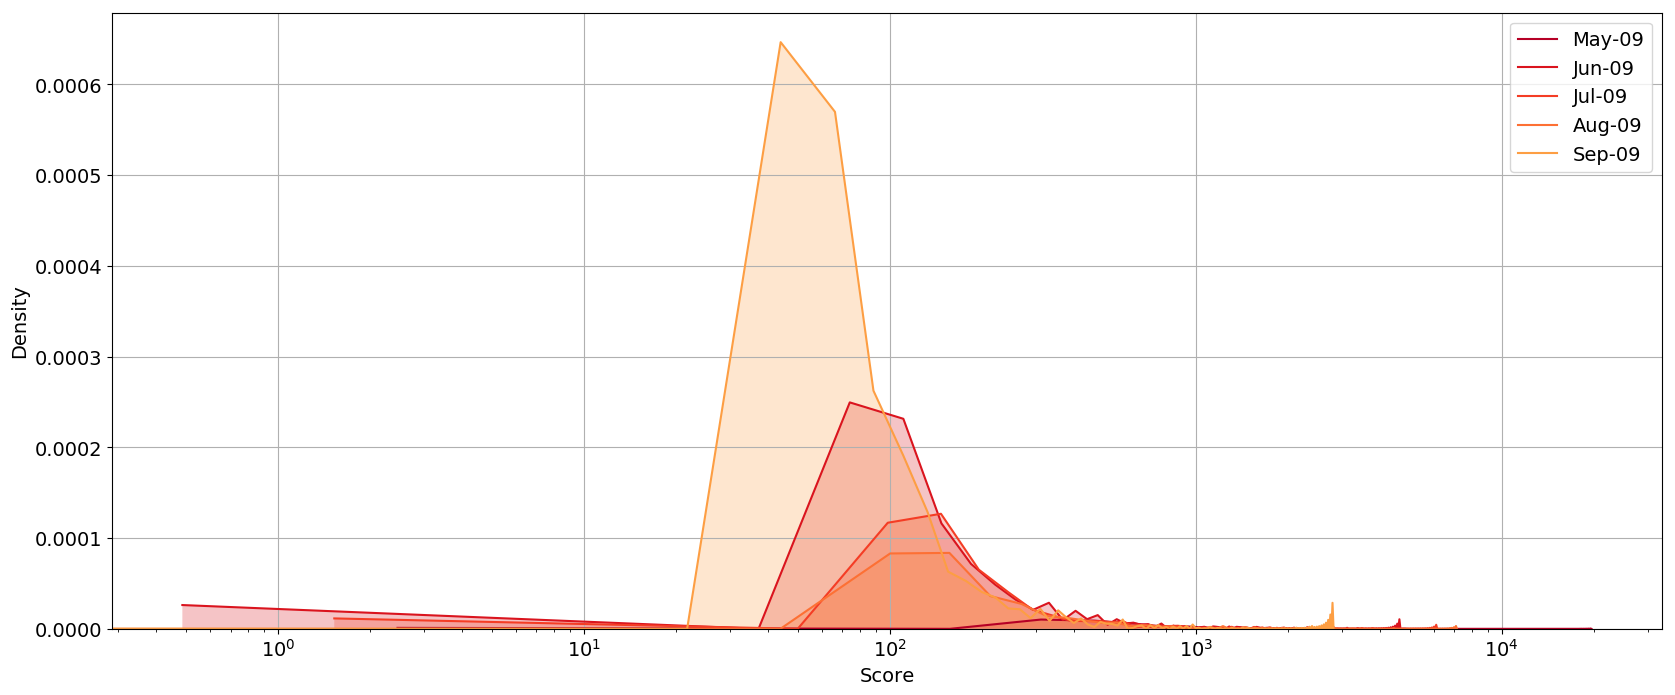
\includegraphics[width=1\linewidth]{../../01-python-code/00-workspace/01-eda/01-graphs/score-sgl-density-plot} \end{center}
\centering {\footnotesize Source: Own calculations in PySpark.}
\end{figure}

\normalsize

\footnotesize

\begin{figure}
\caption{\textbf{ViewCount Variable Density Plot}}
\label{fig:viewc_dens}

\begin{center}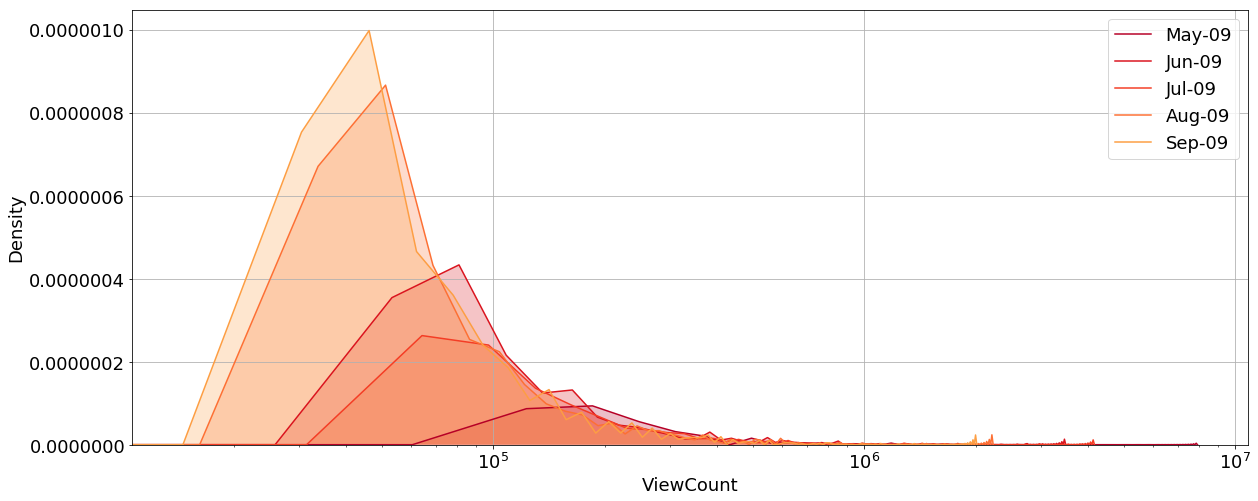
\includegraphics[width=1\linewidth]{../../01-python-code/00-workspace/01-eda/01-graphs/viewcount-sgl-density-plot} \end{center}
\centering {\footnotesize Source: Own calculations in PySpark.}
\end{figure}

\normalsize

In the tables and figures above, we see that the distributions differ
across monthly datasets for both the \texttt{ViewCount} and
\texttt{Score} variables, and both variables appear to be highly
positively skewed. The dataset for May seems to be particularly distinct
from the others, with substantially flatter distributions for both
variables. For the \texttt{Score} variable, the contrasting reputation
levels for up- and down-voting privileges (15 and 125 respectively)
discussed in the previous section no doubt are a primary driver of its
positive skewness. This is due to the fact that if a question is to
receive a vote at all, it is more likely to receive an up-vote.

In light of the positive skewness of both the \texttt{ViewCount} and
\texttt{Score} variables, I opt to take their natural logarithm for the
predictive task. In this way, errors in predicting very high scores and
very low scores will affect the final evaluation metric in the
prediction step equally. The descriptive statistics for the resulting
\texttt{logScore} and \texttt{logViewCount} variables are displayed in
tables \ref{tab:viewcl_desc} and \ref{tab:scorel_desc} below.

\newpage

\footnotesize

\begin{longtable} {@{} lccccc @{}}
\caption{\textbf{logViewCount Variable Descriptive Statistics}}
\label{tab:viewcl_desc}\\ 
\toprule
\textbf{Dataset} & \textbf{Count} & \textbf{Mean} & \textbf{SD} & \textbf{Min} & \textbf{Max} \\ 
\midrule
May-09 &  26\ 026 &   7.8 &     1.7 &  3.3 &  15.9 \\
Jun-09 &  28\ 555 &   7.7 &     1.7 &  3.3 &  15.1 \\
Jul-09 &  32\ 752 &   7.6 &     1.7 &  3.1 &  15.2 \\
Aug-09 &  32\ 998 &   7.5 &     1.7 &  3.1 &  14.6 \\
Sep-09 &  33\ 268 &   7.5 &     1.7 &  3.1 &  14.5 \\
\bottomrule
\end{longtable}\begin{center} Source: Own calculations in PySpark.\end{center}

\normalsize

\footnotesize

\begin{longtable} {@{} lccccc @{}}
\caption{\textbf{logScore Variable Descriptive Statistics}}
\label{tab:scorel_desc}\\ 
\toprule
\textbf{Dataset} & \textbf{Count} & \textbf{Mean} & \textbf{SD} & \textbf{Min} & \textbf{Max} \\ 
\midrule
May-09 &  26\ 026 &   3.4 &     0.4 &  2.8 &  9.9 \\
Jun-09 &  28\ 555 &   3.4 &     0.4 &  2.7 &  8.5 \\
Jul-09 &  32\ 752 &   3.4 &     0.4 &  2.8 &  8.7 \\
Aug-09 &  32\ 998 &   3.4 &     0.4 &  0.7 &  8.9 \\
Sep-09 &  33\ 268 &   3.4 &     0.4 &  2.6 &  7.9 \\
\bottomrule
\end{longtable}\begin{center} Source: Own calculations in PySpark.\end{center}

\normalsize

This finally brings us to a discussion of what the distinction between
the \texttt{Score} and \texttt{ViewCount} variables actually is. We now
know that more views imply a higher \texttt{Score}, owing to the
asymmetrical up- and down-voting privileges, but we don't know if there
is reverse causality as well. An example of this would be questions with
higher \texttt{Scores} spurring on more views as these questions rise to
the top of popular search engines or ``hot question'' lists on the
StackOverflow site.

Regardless of the intricacies of causality between the variables, it is
worth noting that only members that have registered with the community
are able to up-vote and down-vote and thus contribute to the
\texttt{Score}. On the other hand, all questions are open to the public
and therefore the \texttt{ViewCount} variable registers views from 1)
registered users that can vote, 2) registered users that can't vote due
to a reputation level below 15, and 3) non-registered members. This
leads me on to a discussion on the decision of Ravi \emph{et al.} (2014)
to predict on a final response of \texttt{Score} divided by
\texttt{ViewCount}.

Ravi \emph{et al.} (2014) assert that \texttt{ViewCount} is a
measurement of ``popularity'' and thus in order to strictly measure
question quality, divides \texttt{Score} by \texttt{ViewCount} to
mitigate conflating popularity with question quality. I point out
however, that we have no way of knowing what the community-member
composition of the \texttt{ViewCount} for given question is - i.e.~when
normalising by \texttt{ViewCount}, does this divide by a majority of
individuals that can vote, can't vote or a entirely non-registered
members in the community? The assumption of Ravi \emph{et al.} (2014) is
that the composition is a majority of individuals that can vote, which I
believe is not a strong assumption given the popularity of the
StackOverflow site with many non-registered members.

I establish a different framework that I believe is sounder: that of
\emph{within-community} engagement versus \emph{outer-community
engagement}. With these two definitions in mind, it is plain to see that
the \texttt{Score} variable is primarily a within-community engagement
metric since users are required to commit and register with the
StackOverflow community to contribute to this variable by voting.
\texttt{ViewCount} on the other hand can be seen as both a within- and
outer- community engagement variable, because it does not distinguish
between voting or non-voting status when registering question views. One
obvious difference between the two is that the \texttt{Score} variable
is a categorical metric in that users can choose between positive,
negative and neutral engagement, whereas \texttt{ViewCount} only
registers one dimension of engagement (i.e.~whether a question has been
visited or not).

I consequently make the decision to focus solely on within-community
engagement and therefore use the \texttt{Score} variable as it is rather
than normalise by the \texttt{ViewCount} variable. While popularity, or
outer-community engagement, still may influence this variable to some
extent as views drive more registered users to the question who
subsequently vote, I take it as given that having the ability to attract
views is yet another facet of attracting positive community engagement.

The choice of using a continuous \texttt{Score} variable also has two
added benefits. Firstly, there is no need to choose a (potentially)
arbitrary threshold to label good and bad questions for prediction. This
decision in Ravi \emph{et al.} (2014) led to a selection of only 66~388
questions for analysis out of 410~049, or less than 17\%. Lastly, I
believe providing \texttt{Score} predictions over
\texttt{Score}/\texttt{ViewCount} predictions would be more informative
to questioners looking to improve their answers.

The final \texttt{logScore} variable is shown in a boxplot across all
five monthly datasets in figures \ref{fig:score_box}. One last aspect to
note is the significant number of outliers present over the datasets.
Note that we do not want to remove these outliers, but aim to extract
the features that make them so over- and under-valued in the
StackOverflow community.

\footnotesize

\begin{figure}
\caption{\textbf{logScore Variable Box Plot}}
\label{fig:score_box}
\begin{minipage}{1\textwidth}

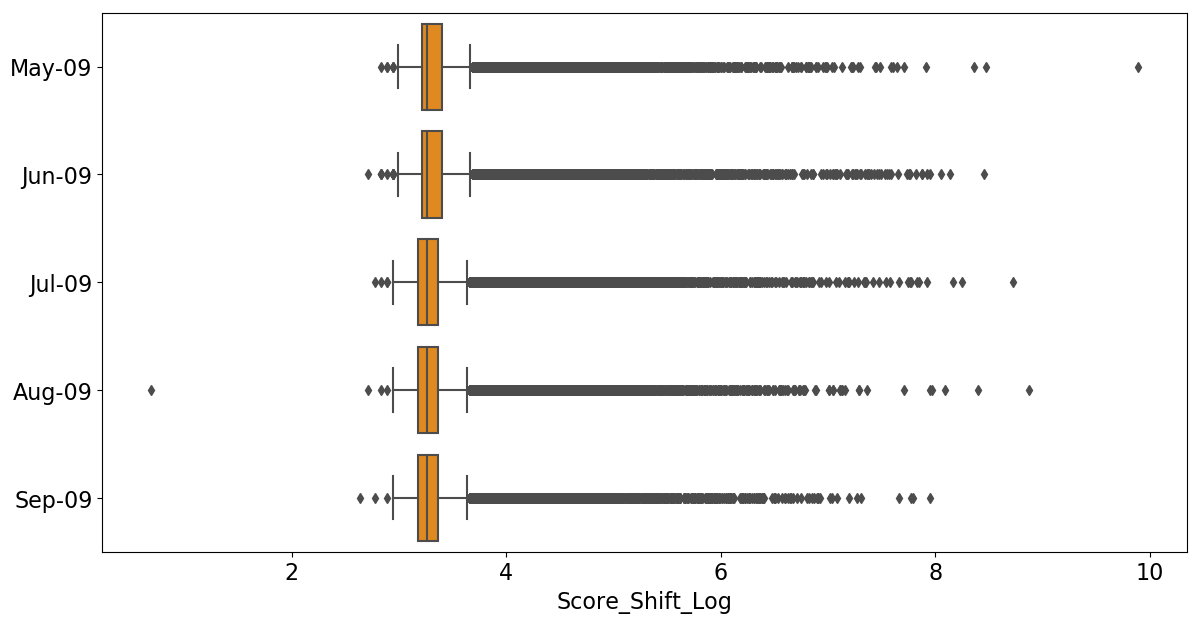
\includegraphics[width=1\linewidth]{../../01-python-code/00-workspace/01-eda/01-graphs/score_shift_log-box-plot} 
\\ \centering
{\footnotesize Source: Own calculations in PySpark.}
\end{minipage}
\end{figure}

\normalsize

\subsubsection{\texorpdfstring{Potential Methodological Issues
\label{Issues}}{Potential Methodological Issues }}\label{potential-methodological-issues}

Two last potential methodological issues are discussed here. Firstly
regarding the \texttt{Score} variable, one potential confounding factor
is that questions can be edited, not only by the original poster, but by
anyone with a reputation of 2~000 or more. General cross-community
guidelines for editing include: addressing grammar and spelling issues,
clarifying concepts, correcting minor mistakes, and adding related
resources and links
(\url{https://stackoverflow.com/help/privileges/edit}). The concern here
is that users could vote, comment and answer on substantially different
questions over time as a question is edited further away from its
original form. The simplifying assumption that I make here is that most
edits, if any at all, happen quickly as moderators and high-reputation
users are made aware of offending questions and thus the majority of
views and votes would happen on final, edited questions. Consequently, I
choose to analyse final edited question content.

A second methodological adjustment that should be considered is the
decision by Ravi \emph{et al.} (2014) to only consider questions above a
certain \texttt{ViewCount} threshold (which they choose to be 1~000).
The reasoning they give for this is to increase their confidence that
the final dataset contains questions that have been viewed by qualifying
users that can vote. Similarly to their decision to normalise their
response variable with \texttt{ViewCount}, I assert that we can not know
if views are contributed by community members that can or can't vote
since there is no data on the distribution of qualifying and
non-qualifying user contributions to views. One could also just as
easily argue that new questions that begin with a low \texttt{ViewCount}
are more likely to see engagement from proactive community members,
especially if these questions don't generate enough webpage activity and
views to rise to the top hit for search engines (which incidentally
would most likely lead to more non-community member contribution to
views). I therefore opt to not disregard any questions below a certain
\texttt{ViewCount} threshold.

\newpage

\subsection{Feature Selection}\label{feature-selection}

The features that I incorporate into the prediction task are extracted
from only the textual content of questions. These features reduce
variable-length documents to fixed-length vectors of real numbers,
essentially numerically summarising documents so that they can be
represented as features with the same dimensions. Common feature
extraction methods include bag-of-words, term frequency-inverse document
frequency (TF-IDF), latent Dirichlet allocation (LDA) and
word-embeddings. Since I focus on textual features of questions only,
all my features are based on the \texttt{Body} and \texttt{Title}
content of questions. I apply the bag-of-words, TF-IDF and latent
Dirichlet allocation feature extraction methods.

\subsubsection{Question Length}\label{question-length}

Length textual features are simple features that can be extracted from
the number of characters, the number of words (or tokens) and the number
of sentences. I will extract these features for both the \texttt{Body}
and \texttt{Title} of each question, which will be used later in a
\emph{length} model in the prediction task.

\subsubsection{Bag-of-words}\label{bag-of-words}

Bag-of-words is a simple textual feature extraction method which maps
documents into \emph{term-frequency} vector. This method does not take
the order of words within a document into account, and if single words
(unigrams) are extracted it does not take into account the co-occurrence
of words. To include the co-occurrence of words, one can extract \(n\)
successive words, or ngrams. Naturally, bag-of-words assumes that the
most relevant information in the document is included in the term
frequency vector.

The bag-of-words method works by splitting each a document into an array
of words or terms (tokenising), and takes their counts as features (with
counts of 0 included) - this is the resulting term frequency vector. In
order to extract these term frequency vectors from the string
\texttt{Body} and \texttt{Title} of questions, I will parse the HTML
content of the \texttt{Body} variable and tokenise lower-case terms from
both the \texttt{Body} and \texttt{Title} content, without punctuation.
I will also remove English stopwords, which are words that are void of
meaning, according to Porter stemming (Porter, 1980).

Once these term frequency vectors have been extracted, each term
frequency for a term is considered a feature, with all the term
frequencies in a term frequency vector representing a document. In this
way, a corpus of documents is represented by a feature matrix with one
row per document and one column per word/term.

\subsubsection{TF-IDF}\label{tf-idf}

Evidently in a large corpus, certain words will occur more often than
others. While it is possible to remove many words that have little to no
meaning (stopwords), the counts in the term frequency vector from
bag-of-words will obviously weight more frequent words, potentially at
the expense of words that are rarer, but more meaningful to the
analysis. One popular method to address this problem is TF-IDF (Salton
and McGill, 1983).

The TF-IDF scheme is a method that re-weights and normalises the term
frequencies and compares them to inverse document frequencies, which are
also suitably normalised. Formally, let \(\text{tf}(t, d)\) denote the
term frequency of a term \(t\) in a document \(d\). The inverse document
frequency for \(t\) is then the following:

\begin{align} \label{eq:idf}
\text{idf}(t) = \log \frac{1 + D}{1 + df(t)}
\end{align}

where \(D\) denotes the total number of documents in the corpus, and
\(df(t)\) denotes the number of documents containing term \(t\).

The TF-IDF vectors \(\text{tf-idf}(t, d)\) are then given by

\begin{align} \label{eq:tf_idf}
\text{tf-idf}(t, d) = \text{tf}(t, d) \times \text{idf}(t)
\end{align}

\newpage

and are finally normalised using the Euclidean norm:

\begin{align} \label{eq:tf_idf_norm}
\text{tf-idf}(t, d)_{norm} = \frac{\text{tf-idf}(t, d)}{ \sqrt{\text{tf-idf}(1, d)^2 + ... + \text{tf-idf}(T, d)^2} }
\end{align}

where \(T\) is the total number of terms in the corpus.

As in bag-of-words, the final result is a term-by-document matrix where
columns now contain normalised TF-IDF values for each document and which
can be used as features for in a predictive model.

\subsubsection{\texorpdfstring{Latent Dirichlet Allocation
\label{lda}}{Latent Dirichlet Allocation }}\label{latent-dirichlet-allocation}

LDA (Blei \emph{et al.}, 2003) is an unsupervised, generative,
three-level hierarchical Bayesian model that can be used to discover the
latent topics in a corpus. LDA assumes that each document is a finite
mixture of a certain number of abstract topics, that each topic is a
discrete probability distribution over words, and that each word is
generated according to one of these topics. In practice, the topics and
other structure are hidden, and so we have to infer them from the
observable documents.

Topic mixtures across documents share a Dirichlet prior, and all word
distributions of topics have another common Dirichlet prior (Blei
\emph{et al.}, 2010). The Dirichlet distribution is a multivariate
generalization of the beta distribution and is useful in facilitating
LDA inference and parameter estimation algorithms because 1) it is in
the exponential family, 2) it has finite dimensional sufficient
statistics, and 3) it is conjugate to the multinomial distribution.
Since Dirichlet distributions are distributions over multinomial
parameter vectors (vectors of positive values that sum to one), they are
also convenient to qualitatively infer what topics represent by
examining the highest probability words per topic.

\newpage

To formalise notation:

\setstretch{0.9}

\begin{itemize}
\item
  Let the the number of assumed topics be denoted \(K\)
\item
  Let the each of the document \(d\) have length \(N_d\), with \(D\)
  questions in the corpus of interest
\item
  Let \(\text{Dir}(a)\) denote the Dirichlet distribution with symmetric
  parameter \(a\)
\end{itemize}

\setstretch{1.5}

The generative process assumed by LDA is then: \newline

\setstretch{0.9}

\textbf{for} each topic \(k = 1, ..., K\) \textbf{do}

\quad Generate word-distribution \(\beta_k \sim \text{Dir}(\gamma)\)

\textbf{end for}

\textbf{for} each document \(d = 1, ..., D\) \textbf{do}

\quad Generate topic-distribution \(\theta_d \sim \text{Dir}(\alpha)\)

\quad \textbf{for} each position \(i = 1, ..., N_d\) in document \(d\)
\textbf{do}

\quad \quad Generate a topic
\(z_{id} \sim \text{Multinomial}(\theta_d)\).

\quad \quad Generate a word
\(w_{id} \sim \text{Multinomial}(\beta_{z_{id}})\).

\quad \textbf{end for}

\textbf{end for} \newline

\setstretch{1.5}

Again, the words \(w_{id}\) are the only variables that are observed,
whereas the topic-document mixtures \(\theta_d\) and topic-word
distributions \(\beta_k\) are latent, or hidden. The Dirichlet priors
for the aforementioned multinomial distributions are \(\alpha\) and
\(\gamma\) respectively, which represent the hyperparameters of the LDA
model.

Since each document has a unique topic mixture, and these topics are
distributions over the corpus vocabulary, LDA can also be viewed as a
mixed membership model. A graphical model representation of LDA is
depicted in figure \ref{fig:lda} below, which highlights the
hierarchical and multi-level structure of the model.

\footnotesize

\begin{figure}
\caption{\textbf{A Probabilistic Graphical Model of LDA}}
\label{fig:lda}

\includegraphics[width=0.8\linewidth]{../../01-python-code/00-workspace/lda-graph-represent} 
\\ 
\centering {\footnotesize Source: Rasmussen (2015). Nodes are random variables, edges indicate dependence and shaded nodes indicate observed variables. Note that in this figure, all documents are assumed to have fixed length $N$.}
\end{figure}

\normalsize

Based on the data generation process above and given the hyperparameters
\(\alpha\) and \(\gamma\), the joint distribution of the topic-word
distribution, topic mixture, topic assignments and words is given by:

\begin{align} \label{eq:posterior}
\text{P}(\beta_{1:K}, \theta_{1:D}, \{z_{id}\}, \{w_{id}\} | \alpha, \gamma) = \prod_{k=1}^K \text{P}(\beta_k | \gamma) \prod_{d=1}^D \left[ \text{P}(\theta_d | \alpha) \prod_{i=1}^{N_d} [\text{P}(z_{id} | \theta_d) \text{P}(w_{id} | \beta_{1:K}, z_{id}) ] \right]
\end{align}

To analyse a corpus, the assumed data generation can be ``reverse
engineered'' by computing the posterior modes of the latent variables
given the words that have been observed. To compute the posterior over
the parameters \(\beta_{1:K}\) and \(\theta_{1:D}\) given the words
\(\{w_{id}\}\) however, we have to marginalise out the latent topic
assignments \(\{z_{id}\}\), and this computation is intractable. This
leaves researchers to call upon approximate posterior inference.

Algorithms that are now available for this inference task include
variational Bayesian (VB) inference proposed in the original paper by
Blei \emph{et al.} (2003), maximum a posteriori estimation (Chien and
Wu, 2008) and collapsed Gibbs sampling which was derived for LDA in
Griffiths and Steyvers (2004). I now move on to a formal discussion of
VB inference.

In VB inference, the true posterior is approximated by a simpler
distribution, \(q(\{z_{id}\}, \eta, \phi)\), which is as close to the
posterior as possible. More specifically, a simpler convex distribution
is used to ascertain a flexible lower bound on the true posterior. The
problematic coupling between \(\theta\) and \(\beta\) parameters are
dropped to make computation tractable. Maximising the lower bound is
equivalent to minimising the Kullback-Leibler (KL) divergence between
\(q(\{z_{id}\}, \eta, \phi)\) and the posterior in \ref{eq:posterior},
where the KL divergence is a measurement of how disparate distributions
are and is given by:

\begin{align} \label{eq:kl}
\text{KL}(f||g) = \sum_{x \in \mathcal{X}} g(x) \log \Big( \frac{f(x)}{g(x)} \Big)
\end{align}

for two distributions \(f\) and \(g\) on a countable set
\(\mathcal{X}\).

Finally, the variational distribution has the bound given in equation
for each document in the corpus \ref{eq:bound}, with the optimisation
equation given in equation \ref{eq:opti}:

\begin{align} \label{eq:bound}
q(\theta, \{z_{id}\}|, \eta, \phi) = q(\theta | \eta) \prod_{i=1}^{N_d} q(\{z_{id}\}|\phi_i)
\end{align}

\begin{align} \label{eq:opti}
(\eta^*, \phi^*)) = \text{arg} \underset{(\eta, \phi)}{\text{min}} \text{D}(q(\theta, \{z_{id}\}|, \eta, \phi) \quad||\quad \text{P}(\theta, \{z_{id}\} | \{w_{id}\}, \alpha, \gamma)) 
\end{align}

The size of the datasets I have chosen to analyse necessitate a
computationally efficient algorithm, of which two modern approaches
stand out: online VB proposed by Hoffman \emph{et al.} (2010), and the
expectation maximisation algorithm developed by Asuncion \emph{et al.}
(2009), both of which can be implemented with the PySpark
\texttt{pyspark.sql.ml.clustering.LDA} package. I will employ the online
VB implementation in Hoffman \emph{et al.} (2010). This technique is
based on online stochastic optimisation, and uses multiple passes to fit
the LDA topic model to a dataset, updating the term-topic distribution
adaptively. Ravi \emph{et al.} (2014) provide a summary of the algorithm
as it relates to this research problem, which is stated below. \newline

\setstretch{0.9}

\textbf{Online LDA Inference Algorithm}

Until converged:

\begin{enumerate}
\def\labelenumi{\arabic{enumi})}
\item
  Randomly choose a mini-batch of questions.
\item
  For each question in the chosen mini-batch:

  \begin{enumerate}
  \def\labelenumii{\alph{enumii})}
  \tightlist
  \item
    Estimate the approximate posterior over which topics each word in
    each question came from
  \end{enumerate}
\item
  Partially update the approximate posterior over the topic
  distributions in accordance with the words that are believed to come
  from specific topics.
\end{enumerate}

\setstretch{1.5}

Online LDA is not only efficient in analysing immense document
collections, but also in dealing with streaming data, which would be
useful to incorporate future questions incrementally on the
StackOverflow site. Having discussed the LDA model and other textual
feature extraction methods, this now brings us to the prediction task.

\newpage

\subsection{\texorpdfstring{Predictive model
\label{Model}}{Predictive model }}\label{predictive-model}

In this section I describe the approach I take in modelling community
engagement in the StackOverflow community, represented by the
\texttt{logScore} variable. Ravi \emph{et al.} (2014) build models with
features from the length, textual content and latent topics of questions
for their binary classification of questions, and my goal is to
investigate whether these models are as effective in predicting
\texttt{logScore} as a measurement of community engagement in a
regression setting.

\subsubsection{Regularised Regression}\label{regularised-regression}

Let \(q_i\) represent question \(i\) out of all questions \(Q\), which
is split into a training set \(Q_\text{train}\) (50\%) and testing set
\(Q_\text{test}\) (50\%). Let \(s_i\) denote the \texttt{logScore} of
each question. Using regularised regression, I predict \(s_i\) using
only features derived from the raw textual \texttt{Body} and
\texttt{Title} of each question, where these features are denoted
\(\bm{x'}_i\). The learning objective therefore, is to find a weight
vector \(\bm{w}\) which minimises the residual sum of squares of the
training corpus \(Q_\text{train}\):

\begin{align} \label{eq:learn_obj}
\underset{\bm{w}}{\text{minimise}} \quad \sum_{ q_{i} \in Q_{\text{train}} } ( s_i - {\bm{w}\bm{x'}_i} )^2  + \lambda \sum_{j=1}^p w_j^2 
\end{align}

where \(\lambda\) is a regularisation parameter to prevent overfitting.

For the prediction task, I employ a grid search over the \(\lambda\)
parameter for a range of 0.001 to 1, and use 2-fold cross validation to
select the best performing model on \(Q_\text{train}\). I choose 2-fold
cross validation since increasing the number of folds had no significant
effect on predictive performance.

\newpage

\subsubsection{Train/Test Split}\label{traintest-split}

One area worth investigating before the prediction task, is potential
heterogeneity in the train and test split, with specific focus on
heterogeneity with regard to time. After randomly splitting \(Q\) into
\(Q_\text{train}\) and \(Q_\text{test}\) of equal sizes, descriptive
statistics for each set are calculated and depicted in table
\ref{tab:rand_tr_te}, rounded to two decimal places.

Table \ref{tab:rand_tr_te} demonstrates that the means and standard
deviations within datasets are similar, with the largest absolute
difference being 0.03 standard deviations in the August dataset. What is
interesting however, is that there is a decreasing trend for both
variables over time from May to August - however whether this is
specific to this data range, or is an indication of downward trends in
the mean and standard deviation of the \texttt{logScore} (and by
implication the \texttt{Score}) variable is unknown. \newline

\footnotesize

\begin{longtable}[htbp] {@{} lcccccc @{}} 
\caption{\textbf{logScore Descriptive Statistics for Random Train/Test Split}} 
\label{tab:rand_tr_te} \\
\toprule
\textbf{Dataset} &  \textbf{Train Mean} &  \textbf{Test Mean} &  \textbf{Train SD} &  \textbf{Test SD} \\
\midrule
May-09 & 3.4 & 3.4 & 0.43 & 0.42 \\
Jun-09 & 3.4 & 3.4 & 0.43 & 0.43 \\
Jul-09 & 3.38 & 3.38 & 0.4 & 0.4 \\
Aug-09 & 3.36 & 3.37 & 0.36 & 0.39 \\
Sep-09 & 3.36 & 3.36 & 0.35 & 0.36 \\
\bottomrule
\end{longtable}\begin{center} Source: Own calculations in PySpark\end{center}

\normalsize

In the interest of robustness I investigate whether there are
substantial differences in means and standard deviations within datasets
for a temporal train/test split. The descriptive statistics for a
temporal train/test split are displayed in table \ref{tab:time_tr_te}
below, again rounded to two decimal places.

While there appears to be a common trend of slightly smaller means and
standard deviations in the test sets for all months, these differences
do not appear to be significantly larger than in the random train/test
split. This at least provides some evidence for my assumption that the
monthly StackOverflow datasets that I have selected are relatively
homogeneous with respect to time. I now use the random train/test split
for the modelling of the \texttt{logScore} variable.

\footnotesize

\begin{longtable}[htbp] {@{} lcccccc @{}} 
\caption{\textbf{logScore Descriptive Statistics for Temporal Train/Test Split}} 
\label{tab:time_tr_te} \\
\toprule
\textbf{Dataset} &  \textbf{Train Mean} &  \textbf{Test Mean} &  \textbf{Train SD} &  \textbf{Test SD} \\
\midrule
May-09 & 3.4 & 3.4 & 0.42 & 0.43 \\
Jun-09 & 3.4 & 3.4 & 0.44 & 0.42 \\
Jul-09 & 3.39 & 3.37 & 0.42 & 0.39 \\
Aug-09 & 3.37 & 3.37 & 0.38 & 0.37 \\
Sep-09 & 3.36 & 3.35 & 0.36 & 0.35 \\
\bottomrule
\end{longtable}\begin{center} Source: Own calculations in PySpark\end{center}

\normalsize

\subsubsection{Features}\label{features}

I use the \texttt{Body} and \texttt{Title} content of questions as
separate signals for feature extraction in the StackOverflow community.
I extract numerical length features on both the pre-processed
\texttt{Body} and \texttt{Title} variables, employ bag-of-words feature
extraction to ascertain term frequency vector features and also
translate these into TF-IDF features. I use only unigram features for
the bag-of-words and TF-IDF feature extraction, since there were no
improvements in performance for higher order ngrams from a held out
dataset in the predictive task.

As discussed by Ravi \emph{et al.} (2014), there are a number of aspects
that could define a good question, or in the framework presented here, a
question that is highly valued by the StackOverflow community.
Bag-of-words and TF-IDF may capture certain aspects about questions that
are stated particularly clearly or that show prior research through the
mentioning of key words, but there are also other more subtler aspects
of questions, such as topical relevance, that could signal question
constructiveness.

Evidently, a range of overall topics is discussed in the StackOverflow
community every day, week, month and so on. Ravi \emph{et al.} (2014)
assert that there may be community engagement variation along these
topics due to 1) differing behaviour of sub-communities in terms of how
up- and down-votes are attributed to questions about specific topics,
and 2) questions concerning popular versus unpopular topics receiving
varying degrees of community engagement. They use this as a motivation
for including features in their prediction task relating to ``global''
topic information - global here meaning that these topics reflect what
entire questions are about. Since these global topics from questions in
the StackOverflow community can be extracted in an unsupervised way with
latent topic models, they employ LDA to do precisely this.

I employ global the LDA topic model from Ravi \emph{et al.} (2014), and
train the online LDA model (Hoffman \emph{et al.}, 2010) over all
questions \(Q\). I choose \(K=10\) topics and sparse Dirichlet priors,
setting hyperparameters \(\gamma\) and \(\alpha\) to a value of 0.01 to
encourage the learning of fewer topics per question and sparser
topic-word distributions. For each question \(q_i \in Q\), I add a
feature for topic \(k\) with weight \(\theta_{q_ik}\) (the inferred
topic mixture for question \(q_i\)), resulting in 10 features
\((\theta_{q_i1}, \theta_{q_i2}, ..., \theta_{q_i{10}})\) being
incorporated for the prediction task per question.

Table \ref{tab:top_words} shows the top three words per dataset for the
10 sample topics learned in the global LDA model. While these words can
help the researcher interpret what the topics concern qualitatively, the
true topics will still remain unknown to us. In table
\ref{tab:top_words} we see a range of words that are intuitive, such as
\emph{file}, \emph{system}, \emph{twitter} and \emph{socket} etc., as
well as words that evidently relate to code extracts in the
StackOverflow questions like \emph{div}, \emph{std}, \emph{id}, and
\emph{class}. Computer programming languages that the topics appear to
be capturing over the monthly datasets include Java, PHP, Ruby, Python
and the distributed version-control system Git. All in all, it does
appear as if the global LDA model is capturing the ``aboutness'' of
questions to some extent.

\begin{landscape}

\vspace*{70px}

\footnotesize
\begin{longtable}[htbp] {@{} cccccc @{}} 
\caption{\textbf{Top Words of Global LDA Sample Topics}} 
\label{tab:top_words} \\
\toprule
\textbf{Topic} &  \textbf{May 2009} & \textbf{June 2009} & \textbf{July 2009} & \textbf{August 2009} & \textbf{September 2009} \\
\midrule
T1 & amp quot lib &    imagenam   usernam  dim & file          use   system   &       amp      mx   twitter & imag   menuviewcontrol   socket \\
T2 & myclass round treeview & xs width height &  helloworld         self      amp   & file    user     class &  lib               gem     rubi \\ 
T3 & nhibern station buffer & node   neutral   publickeytoken &   po   objnicitem   public    & char      th       org & public            string      xsd \\ 
T4 & xxx java assembl &    countri    branch             span &    amp         nbsp       me   & self     std       int & sbquo              task      amp \\ 
T5 & xsd wsdl anim &         div       std id & int       string      std & boost     xsl    system & java               org   eclips \\ 
T6 & control imag public &        lib       gem               rb &  java          org   hibern & div      id       php & class              file       id \\ 
T7 & id div tabl &         id    select             tabl &  py         date     cout & option    valu      woot &    system             param      dll \\
T8 & file string server &      java       xsl             file &  param       string   thread &  width      id      nbsp & mx            unsign   hibern \\     
T9 & encrypt system http &     cach     dword              age & div         text       id &  xs     org    schema & id        routecount      git \\
T10 & java org defaultactioninvoc &       int      list class &   bf          xsl       xs & java   apach       org &  xsl   menuviewcontrol     cell \\ 
\bottomrule
\end{longtable}
\begin{center} Source: Own calculations in PySpark\end{center}
\normalsize


\end{landscape}

\subsubsection{\texorpdfstring{Evaluation
\label{eval}}{Evaluation }}\label{evaluation}

A question that still remains is what evaluation metric to use to
compare across models and across datasets. Both the mean absolute error
(MAE) and the root mean square error (RMSE) are frequently employed as
model evaluation metrics in the broad literature, but as statistics that
condense and summarise the data into a single value, they characterise
model performance error characteristics in decidedly distinct manners.

Criticisms have been laid against RMSE asserting that 1) it does not
indicate average model performance well and may be a misleading
indicator of average error (Willmott and Matsuura, 2005), and 2) it is
ambiguous in interpretation because as a sums-of-squares-based statistic
it does not satisfy the triangle inequality for distance metrics
(Willmott \emph{et al.}, 2009). Chai and Draxler (2014) demonstrate
however that RMSE does satisfy the triangle inequality requirement
however, and thus confirm that RMSE is not ambiguous in meaning.

Contrary to the assertion that RMSE does not describe average model
performance well, Chai and Draxler (2014) go on further to affirm that
RMSE is actually a more appropriate metric over MAE when the error
distribution of the model is expected to be Gaussian instead of uniform,
and when there are sufficient samples. They note that while RMSE is more
sensitive to outliers, the Gaussian distribution describes the existence
and probability of outliers well and moreover, since RMSE gives more
weight to unfavourable conditions, it may discriminate better between
model performance differences.

In light of the findings of Chai and Draxler (2014), I choose to use
RMSE to evaluate model performance. Firstly, my sample sizes are not
small, ranging from 26~026 to 33~268. Secondly, the large number of
outliers identified in the \texttt{logScore} variable and depicted in
figure \ref{fig:score_box} in section \ref{scorevc_vis} are indeed not
anomalies in the data, but are highly valuable data points because of
the extent to which the StackOverflow community engages positively or
negatively with these questions. I therefore believe that a higher
weighting for these points is not problematic. Lastly, I assume that the
error distributions of models for the \texttt{logScore} variable are
more likely be Gaussian as opposed to uniform.

\newpage

\section{\texorpdfstring{Results
\label{Results}}{Results }}\label{results}

In order to be able to draw some comparisons of how well the predictive
models are faring, I establish both a low and high benchmark for
predictive performance on the \texttt{logScore} variable. The low
benchmark consists of using the mean of \texttt{logScore} in the
training set as the prediction for every question in the test set, and
the high benchmark uses the \texttt{logViewCount} variable alone to
predict on \texttt{logScore}.

Figures \ref{fig:may_res} to \ref{fig:sept_res} display the training and
test RMSE results for each model employed. The following models are
listed from left to right on the x-axis:

\setstretch{0.9}

\begin{itemize}
\item
  The constant mean baseline
\item
  The length model, which includes features derived from token counts,
  sentence counts and character counts
\item
  The bag-of-words model (which Ravi \emph{et al.} (2014) refer to as
  the \emph{text} model)
\item
  The TF-IDF model
\item
  The global LDA topic model, which includes inferred latent topic
  mixtures
\item
  A final combined model which incorporates features from both the
  length and topic models (but not bag-of-words or TF-IDF)
\item
  The high benchmark model with \texttt{logViewCount} as a single
  feature (note that this model is vacuous since the \texttt{ViewCount}
  variable is not available for new questions)
\end{itemize}

\setstretch{1.5}

\footnotesize

\begin{figure}
\caption{\textbf{Model Training and Test RMSEs for May 2009}}
\label{fig:may_res}

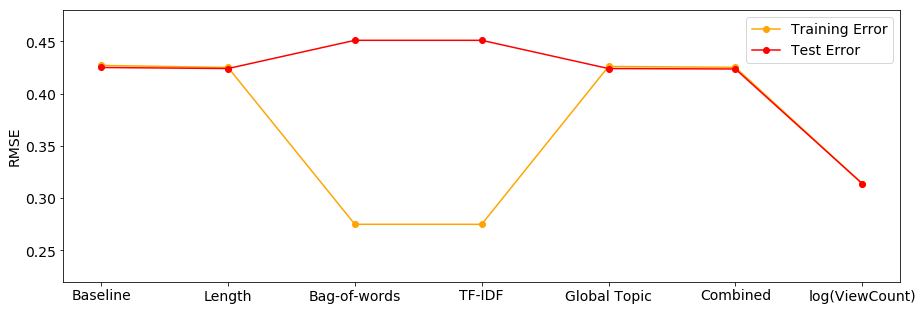
\includegraphics[width=1\linewidth]{../../01-python-code/00-workspace/01-eda/01-graphs/May-09-rmse-results} 
\centering {\footnotesize Source: Own calculations in PySpark.}
\end{figure}

\normalsize

\footnotesize

\begin{figure}
\caption{\textbf{Model Training and Test RMSEs for June 2009}}
\label{fig:jun_res}

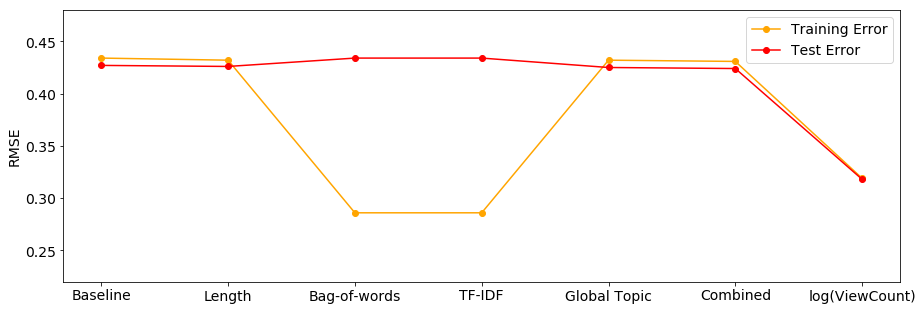
\includegraphics[width=1\linewidth]{../../01-python-code/00-workspace/01-eda/01-graphs/Jun-09-rmse-results} 
\end{figure}

\normalsize

\footnotesize

\begin{figure}
\caption{\textbf{Model Training and Test RMSEs for July 2009}}
\label{fig:jul_res}

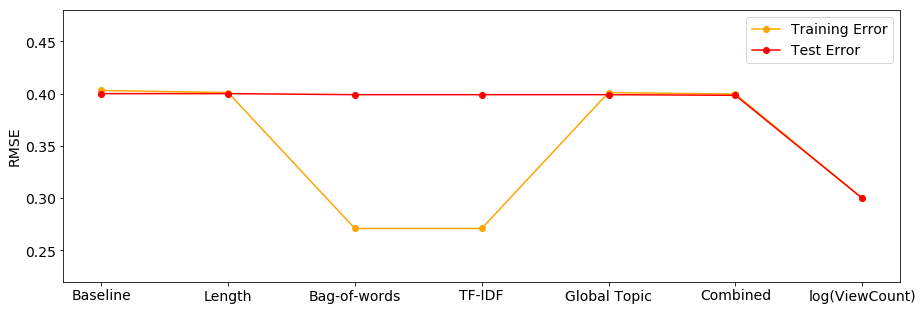
\includegraphics[width=1\linewidth]{../../01-python-code/00-workspace/01-eda/01-graphs/Jul-09-rmse-results} 
\end{figure}

\normalsize

\footnotesize

\begin{figure}
\caption{\textbf{Model Training and Test RMSEs for August 2009}}
\label{fig:aug_res}

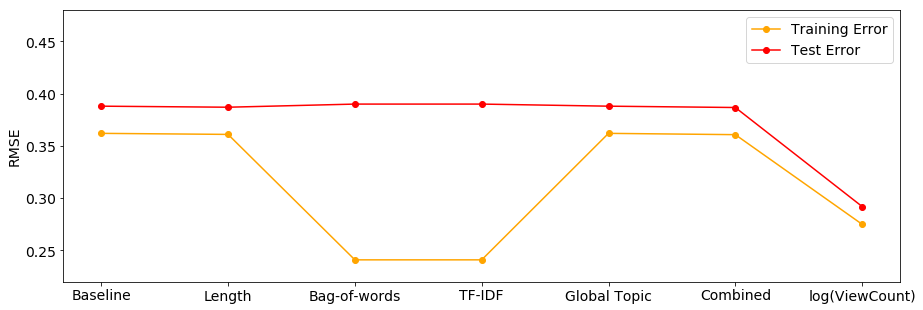
\includegraphics[width=1\linewidth]{../../01-python-code/00-workspace/01-eda/01-graphs/Aug-09-rmse-results} 
\centering {\footnotesize Source: Own calculations in PySpark.}
\end{figure}

\normalsize

\footnotesize

\begin{figure}
\caption{\textbf{Model Training and Test RMSEs for September 2009}}
\label{fig:sept_res}

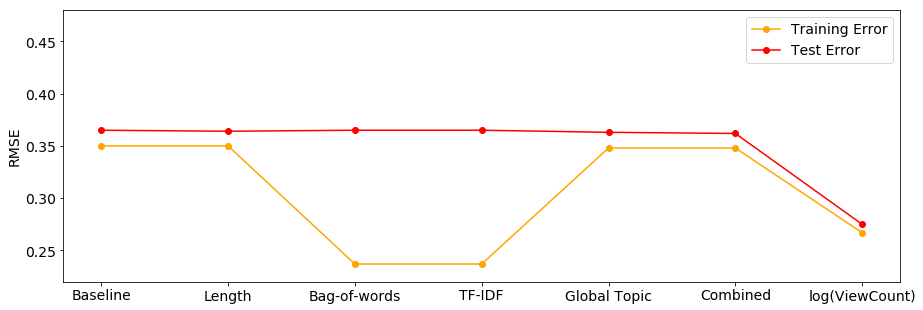
\includegraphics[width=1\linewidth]{../../01-python-code/00-workspace/01-eda/01-graphs/Sep-09-rmse-results} 
\centering {\footnotesize Source: Own calculations in PySpark.}
\end{figure}

\normalsize

The most striking result across all monthly datasets is how consistent
the results are for the test RMSE on all models except for the
\texttt{logViewCount} model, which beats out the baseline with a
reduction of around 25\% in RMSE for all five monthly datasets. This
high performance is analogous with the high correlations between
\texttt{Score} and \texttt{ViewCount} seen in table \ref{tab:corr} in
section \ref{scorevc_vis}. The other models besides the
\texttt{logViewCount} model show no improvement in test RSME over the
baseline, which leads to model test RMSEs mirroring the test set
standard deviations seen in table \ref{tab:rand_tr_te}, since the models
are performing no better than a constant mean prediction on the test
set.

For the training error curves, we again see consistent results in the
length, global topic and combined model, but significantly lower
training errors for the bag-of-words and TF-IDF models. Test RMSE for
the bag-of-words and TF-IDF models is marginally higher than the
baseline for September and August, but substantially higher in May and
June, demonstrating a prevalence of overfitting for these models, since
this implies \emph{worse} performance than constant training mean
prediction.

Interestingly, we see that the test RMSE coincides or is lower than
training RMSE for all models across the May, June and July datasets. If
we re-examine table \ref{tab:rand_tr_te} in section \ref{eval} however,
we see the reason for the lower test error curves is that the standard
deviations of the test set are lower than the training set while the
means are almost identical. Thus, by predicting the same mean for both
sets but where the test set has less variance, the result will naturally
be a lower test RMSE.

Evidently, none of the textual features extracted appear to be good
predictors of the \texttt{logScore} variable in this regression setting
- the models do not appear to be learning specific key words, weighted
or otherwise, nor topics identified by the global LDA model that
differentiate between positive and negative community engagement. These
results thus give us the answer to the research question stated in
section \ref{Intro}, namely that with the textual question content
features that I extracted in this framework, I am \emph{not} able to
predict the \texttt{logScore} variable as a measurement of online Q\&A
community engagement with question content alone.

Recall that Ravi \emph{et al.} (2014) achieved a classification accuracy
of 55.5\% for their length model, 65.8\% in their text model, 64.2\% in
their global topic model and 70.5\% in their combined model with all
three types of features obtains (text included), all above a benchmark
of 61.1\% for their \texttt{ViewCount} model. Having extracted questions
from the same online Q\&A community and time period as Ravi \emph{et
al.} (2014), the differences in our methodologies were 1) I predict on
the \texttt{logScore} variable rather than
\texttt{Score}/\texttt{ViewCount}, 2) I employ a regression model rather
than classification, and 3) I use all the data from monthly time frame,
instead of a subset of the data.

While direct comparison to the results of Ravi \emph{et al.} (2014) is
limited owing to the aforementioned methodological extensions, my
results starkly contrast the same question content models Ravi \emph{et
al.} (2014) employed. A particular aspect to point out is that the
\texttt{ViewCount} model in Ravi \emph{et al.} (2014) was outperformed
by the majority of their models, however the results above show that the
\texttt{logViewCount} model outperforms by a very strong margin.

Ostensibly, accurately predicting a continuous measurement of community
engagement from question content alone in a regression setting is an
ambitious task, and a task which may not see the success of the likes of
the classification model employed in Ravi \emph{et al.} (2014).
Nevertheless, I believe it is a useful framework in the interest of
providing continuous community engagement predictions to questioners,
upon which further research may investigate. This brings me onto how I
believe future research can improve upon the results presented here.

\newpage

\section{\texorpdfstring{Recommendations for Further Research
\label{Recom}}{Recommendations for Further Research }}\label{recommendations-for-further-research}

\subsection{Improving Methodological
Robustness}\label{improving-methodological-robustness}

For recommended areas of further research, I first discuss
methodological improvements that I believe would benefit the analysis.
In section \ref{Issues}, I mentioned some potential issues regarding
some finer nuances in the functioning of the StackOverflow website. Out
of these limitations, the permitted editing of questions stands out as
the strongest methodological limitation. As a reminder, questions can be
edited not only by the original questioner, but by any community member
with 2~000 reputation or more. This means that community members could
view and vote on edited questions that are fundamentally different from
the original question. While I assumed that this editing was minimal and
took place quickly so that very few views and votes were cast on
previous versions of questions, suggestions for further research would
be investigating 1) how much editing takes place over questions, 2) the
time taken until edits versus votes cast and views accumulated, and 3)
how evenly editing is distributed over questions.

As discussed in detail in section \ref{Vars}, there are other options
for community engagement besides the \texttt{Score} variable, each with
their own advantages and disadvantages. While I believe I thoroughly
justified and validated my choice of the \texttt{Score} variable as an
objective and informative response, a thorough exploration of community
engagement measurements in different research frameworks may prove
fruitful, especially of binary metrics in a classification setting given
that prediction in a regression setting here was unsuccessful.
Furthermore, Ravi \emph{et al.} (2014) claim that their methods are
applicable to other Q\&A platforms given that they do not rely on
domain-specific knowledge. Consequently, it may well be worthwhile to
replicate both Ravi \emph{et al.} (2014) and my analysis on other Q\&A
communities to gain insight into how our predictive models fare there.

Lastly, although temporal aspects of the data were discussed thoroughly
in this paper, I believe this is still a prominent area for further
analysis. Further research could investigate the extent to which older
questions are biased to have higher \texttt{Scores} and
\texttt{ViewCounts}, and what the main sources of potential bias are
(i.e.~time, questioner variation, community variation or
community-structure variation). I am of the opinion that: the types of
questioners asking questions, the way in which questioners ask
questions, the composition of the StackOverflow community and overall
community engagement behaviour, have all varied substantially over the
many years that StackOverflow has been active. This would suggest that
any model aiming to predict future community engagement in online Q\&A
fora must be expanded to include time-series elements (regardless of how
short the time span of the data is). This brings me to additional
techniques that could improve on the predictive performance in this
paper.

\subsection{Improving Model
Performance}\label{improving-model-performance}

Although the equally poor results of the diverse textual feature models
in this paper hint that further feature engineering may not
significantly improve model performance, there are a number of more
sophisticated feature engineering methods available to employ that may
yet yield improvements. Ravi \emph{et al.} (2014) assert that, in
addition to global topic models, local topic models may also contain
useful information for predicting community engagement. The authors
implement two such models that relate to the internal structure of
questions such as demonstrating aspects of prior research, a problem
statement, reproducible code, and so on.

Ravi \emph{et al.} (2014) follow the work done by Brody and Elhadad
(2010) on capturing local document aspects with LDA models over
sentences and employ a local sentence-level model to capture certain
aspects within questions. For the model with features from local
sentence-level topics in Ravi \emph{et al.} (2014), they obtain a
classification accuracy 61.4\%. The last LDA model employed by Ravi
\emph{et al.} (2014) is a generalized Mallows (Fligner and Verducci,
1986) global topic structure model. This model aims to capture
discourse-level properties such as adjacent sentences sharing the same
topics and related questions with comparable topics in similar orders,
however yields only 55.6\% accuracy. I believe that the extraction,
evaluation and comparison of models with these features to the those in
this paper would prove insightful.

Blei \emph{et al.} (2010) note that a key limitation for LDA is that it
requires the number of topics to be fixed in advance. Further research
can also therefore explore the most prudent choice for the number of
topics, \(K\), possibly by examining predictive fits on held out
documents, or by selecting the value based on the marginal probability
of the corpus.

Other feature engineering techniques that stand out as areas of further
research include word-embeddings introduced by Mikolov \emph{et al.}
(2013), and even simple dictionary methods that identify sentiment and
emotional language. The substantial literature on outliers and outlier
detection was also not discussed in this paper, yet owing to the
appearance of the numerous outliers in the StackOverflow data, this is
seemingly a field ripe for investigation. Lastly, I believe that a major
room for improvement concerns the predictive model employed in the
regression setting of this paper. I leave it to further research to
explore more complex predictive models in both the classification
setting of Ravi \emph{et al.} (2014) and the regression setting here, to
ascertain if question content can predict a measure of community
engagement with some accuracy.

\newpage

\section{\texorpdfstring{Concluding Remarks
\label{Concl}}{Concluding Remarks }}\label{concluding-remarks}

The goal of this paper was to build on a relatively unstudied area of
research and to test previously successful predictive question content
models on a continuous, comprehensive and objective measurement of
online community engagement. This objective has a valuable use-case,
namely to provide questioners in online Q\&A communities with real-time
predictions of how positively a community will engage with their
question, therefore allowing them to improve their questions before
adding demand to expert resources in a community.

In the context of the StackOverflow community, I showed that the
\texttt{Score} variable is an ideal measure of community engagement for
three reasons. First, it is a primary function of the community.
Secondly, it is able to register both negative and positive community
engagement. Third, it is highly informative. Importantly, the
methodology presented here can be implemented on more diverse online
community datasets for evaluation: the \texttt{Score} variable is
available across all of the 174 StackExchange communities, and similar
metrics can be found on other Q\&A platforms like Quora, MOOCS and so
on.

The main extension of the analysis in Ravi \emph{et al.} (2014) that I
made was to predict on a continuous measurement for community engagement
in a regression setting, rather than classification of binary categories
of questions. I also touched on the aspect of temporality in online Q\&A
communities that has yet to be considered in the literature. I asserted
that there are almost certainly temporal trends inherent in online Q\&A
data extracted from long time periods and thus chose to analyse data
over monthly time periods in order to mitigate potential problems
relating to temporality. Lastly, I used all question data within my
selected time period, compared to Ravi \emph{et al.} (2014) who selected
a subset of around 16\% from questions extracted over a year.

My results fared poorly for models with features engineered from
question content, especially regarding the performance of models in Ravi
\emph{et al.} (2014) in their framework, who found that question content
models performed substantially better than a strong baseline. I found
that question length, textual-content and latent topic models had no
better performance in RMSE than a trivial benchmark of constant training
mean prediction, and also found that a model including only the
\texttt{logViewCount} variable outperformed all other models
significantly. In light of the poor predictive performance of the models
employed in this paper, I recommend future work explore more
sophisticated predictive models and textual feature engineering, as well
as other binary community engagement variables in a classification
setting.

Predicting on a continuous measurement of community engagement using
only question content is evidently an ambitious goal. To the best of my
knowledge, no prior research has endeavoured to capture and predict
community engagement in this regard, and so at the very least this
research has taken a humble step forward in predicting online community
engagement in real time. I leave it to future research to extend the
methodology that I have developed here, with the possibility of
significantly enhancing the functioning of all online Q\&A communities
by accurately predicting online Q\&A community engagement.

\newpage

\section*{References}\label{references}
\addcontentsline{toc}{section}{References}

\hypertarget{refs}{}
\hypertarget{ref-Agichtein2008}{}
Agichtein, E., Castillo, C., Donato, D., Gionis, A. and Mishne, G.
(2008) `Finding high-quality content in social media', in
\emph{Proceedings of the 2008 international conference on web search and
data mining}, pp. 183--194. doi:
\href{https://doi.org/10.1145/1341531.1341557}{10.1145/1341531.1341557}.

\hypertarget{ref-Alexa.com2019}{}
Alexa.com (2019) `The top 500 sites on the web'. Available at:
\url{https://www.alexa.com/topsites}.

\hypertarget{ref-Allamanis2013}{}
Allamanis, M. and Sutton, C. (2013) `Why, when, and what: Analyzing
stack overflow questions by topic, type, and code', in \emph{2013 10th
working conference on mining software repositories (msr)}. IEEE, pp.
53--56. doi:
\href{https://doi.org/10.1109/MSR.2013.6624004}{10.1109/MSR.2013.6624004}.

\hypertarget{ref-Anderson2012}{}
Anderson, A., Huttenlocher, D., Kleinberg, J. and Leskovec, J. (2012)
`Discovering value from community activity on focused question answering
sites: a case study of stack overflow', in \emph{KDD}. ACM, pp.
850--858. Available at: \url{http://dl.acm.org/citation.cfm?id=2339665}.

\hypertarget{ref-Asuncion2009}{}
Asuncion, A., Welling, M., Smyth, P. and Teh, Y. W. (2009) `On smoothing
and inference for topic models', in \emph{Proceedings of the 25th
conference on uncertainty in artificial intelligence}. AUAI Press, pp.
27--34.

\hypertarget{ref-Bian2009}{}
Bian, J., Liu, Y., Zhou, D., Agichtein, E. and Zha, H. (2009) `Learning
to recognize reliable users and content in social media with coupled
mutual reinforcement', in \emph{Proceedings of the 18th international
conference on world wide web}, pp. 51--60. doi:
\href{https://doi.org/10.1145/1526709.1526717}{10.1145/1526709.1526717}.

\hypertarget{ref-Blei2003}{}
Blei, D. M., Ng, A. Y. and Jordan, M. I. (2003) `Latent Dirichlet
Allocation', \emph{Journal of Machine Learning Research}, 3, pp.
993--1022.

\hypertarget{ref-Blei2010}{}
Blei, D., Carin, L. and Dunson, D. (2010) `Probabilistic Topic Models: A
focus on graphical model design and applications to document and image
analysis', \emph{IEEE signal processing magazine}, 27(6), pp. 55--65.
doi: \href{https://doi.org/10.1038/jid.2014.371}{10.1038/jid.2014.371}.

\hypertarget{ref-Brody2010}{}
Brody, S. and Elhadad, N. (2010) `An unsupervised aspect-sentiment model
for online reviews', in \emph{HLT/naacl}. Association for Computational
Linguistics, pp. 804--812.

\hypertarget{ref-Chai2014}{}
Chai, T. and Draxler, R. R. (2014) `Root mean square error (RMSE) or
mean absolute error (MAE)? - Arguments against avoiding RMSE in the
literature', \emph{Geoscientific Model Development}, 7(3), pp.
1247--1250. doi:
\href{https://doi.org/10.5194/gmd-7-1247-2014}{10.5194/gmd-7-1247-2014}.

\hypertarget{ref-Chiang2010}{}
Chiang, D., Graehl, J., Knight, K., Pauls, A. and Ravi, S. (2010)
`Bayesian Inference for Finite-State Transducers', in \emph{HLT/naacl},
pp. 447--455.

\hypertarget{ref-Chien2008}{}
Chien, J. T. and Wu, M. S. (2008) `Adaptive Bayesian latent semantic
analysis', \emph{IEEE Transactions on Audio, Speech and Language
Processing}, 16(1), pp. 198--207. doi:
\href{https://doi.org/10.1109/TASL.2007.909452}{10.1109/TASL.2007.909452}.

\hypertarget{ref-Daume2006}{}
Daumé, H. and Marcu, D. (2006) `Bayesian query-focused summarization',
\emph{ACL}, 1, pp. 305--312.

\hypertarget{ref-Eppler2004}{}
Eppler, M. J. and Mengis, J. (2004) `The concept of information
overload: A review of literature from organization science, accounting,
marketing, MIS, and related disciplines', \emph{Information Society},
20(5), pp. 325--344. doi:
\href{https://doi.org/10.1080/01972240490507974}{10.1080/01972240490507974}.

\hypertarget{ref-Fligner1986}{}
Fligner, M. and Verducci, J. S. (1986) `Distance based ranking models',
\emph{Journal of the Royal Statistical Society: Series B
(Methodological)}, 48(3), pp. 359--369.

\hypertarget{ref-Griffiths2004}{}
Griffiths, T. L. and Steyvers, M. (2004) `Finding scientific topics',
\emph{Proceedings of the National Academy of Sciences of the United
States of America}, 101(SUPPL. 1), pp. 5228--5235. doi:
\href{https://doi.org/10.1073/pnas.0307752101}{10.1073/pnas.0307752101}.

\hypertarget{ref-Haghighi2010}{}
Haghighi, A. and Klein, D. (2010) `Coreference Resolution in a Modular,
Entity-Centered Model', in \emph{HLT/naacl}, pp. 385--393.

\hypertarget{ref-Hoffman2010}{}
Hoffman, M. D., Blei, D. M. and Bach, F. (2010) `Online Learning for
latent Dirichlet allocation (Supplementary Material)', \emph{Nature},
pp. 1--9. doi: \href{https://doi.org/10.1.1.187.1883}{10.1.1.187.1883}.

\hypertarget{ref-Jeon2006}{}
Jeon, J., Croft, W. B., Lee, J. H. and Park, S. (2006) `A framework to
predict the quality of answers with non-textual features', in
\emph{SIGIR}, pp. 228--235. doi:
\href{https://doi.org/10.1145/1148170.1148212}{10.1145/1148170.1148212}.

\hypertarget{ref-Kozareva2011}{}
Kozareva, Z. and Ravi, S. (2011) `Unsupervised name ambiguity resolution
using a generative model', in \emph{Proc. 1st workshop on unsupervised
learning in nlp}, pp. 105--112. Available at:
\url{http://dl.acm.org/citation.cfm?id=2140471}.

\hypertarget{ref-Li2010}{}
Li, B. and King, I. (2010) `Routing questions to appropriate answerers
in community question answering services', in \emph{CIKM}, pp.
1585--1588. doi:
\href{https://doi.org/10.1145/1871437.1871678}{10.1145/1871437.1871678}.

\hypertarget{ref-Li2012}{}
Li, B., Jin, T., Lyu, M. R., King, I. and Mak, B. (2012) `Analyzing and
predicting question quality in community question answering services',
in \emph{WWW companion}, pp. 775--782. doi:
\href{https://doi.org/10.1145/2187980.2188200}{10.1145/2187980.2188200}.

\hypertarget{ref-Li2011}{}
Li, B., King, I. and Lyu, M. R. (2011) `Question routing in community
question answering', in \emph{CIKM}, pp. 2041--2044. doi:
\href{https://doi.org/10.1145/2063576.2063885}{10.1145/2063576.2063885}.

\hypertarget{ref-Liu2008}{}
Liu, Y., Bian, J. and Agichtein, E. (2008) `Predicting information
seeker satisfaction in community question answering', in \emph{SIGIR},
pp. 483--490. doi:
\href{https://doi.org/10.1145/1390334.1390417}{10.1145/1390334.1390417}.

\hypertarget{ref-Mikolov2013}{}
Mikolov, T., Chen, K., Corrado, G. and Dean, J. (2013) `Efficient
Estimation of Word Representations in Vector Space', pp. 1--12.
Available at: \url{http://arxiv.org/abs/1301.3781}.

\hypertarget{ref-Porter1980}{}
Porter, M. F. (1980) `An algorithm for suffix stripping',
\emph{Program}, 14(3), pp. 130--137.

\hypertarget{ref-Qu2009}{}
Qu, M., Qiu, G., He, X., Zhang, C., Wu, H., Bu, J. and Chen, C. (2009)
`Probabilistic question recommendation for question answering
communities', in \emph{WWW}, pp. 1229--1230. doi:
\href{https://doi.org/10.1145/1526709.1526942}{10.1145/1526709.1526942}.

\hypertarget{ref-Ravi2014}{}
Ravi, S., Pang, B., Rastogi, V. and Kumar, R. (2014) `Great Question!
Question Quality in Community Q\&A', in \emph{Eighth international aaai
conference on weblogs and social media}. (1), pp. 426--435.

\hypertarget{ref-Reisinger2009}{}
Reisinger, J. and Paşca, M. (2009) `Latent variable models of
concept-attribute attachment', in \emph{ACL/ijcnlp}, pp. 620--628. doi:
\href{https://doi.org/10.3115/1690219.1690233}{10.3115/1690219.1690233}.

\hypertarget{ref-Riahi2012}{}
Riahi, F., Zolaktaf, Z., Shafiei, M. and Milios, E. (2012) `Finding
expert users in community question answering', in \emph{WWW companion},
pp. 791--798. doi:
\href{https://doi.org/10.1145/2187980.2188202}{10.1145/2187980.2188202}.

\hypertarget{ref-Ritter2010}{}
Ritter, A., Mausam and Etzioni, O. (2010) `A latent dirichlet allocation
method for selectional preferences', \emph{ACL}, (July), pp. 424--434.

\hypertarget{ref-Salton1983}{}
Salton, G. and McGill, M. (1983) \emph{Introduction to modern
information retrieval}. Mcgraw-Hill.

\hypertarget{ref-Shah2010}{}
Shah, C. and Pomerantz, J. (2010) `Evaluating and predicting answer
quality in community QA', in \emph{SIGIR}, pp. 411--418. doi:
\href{https://doi.org/10.1145/1835449.1835518}{10.1145/1835449.1835518}.

\hypertarget{ref-Shah2018}{}
Shah, V., Gulikers, L., Massoulié, L. and Vojnović, M. (2018) `Adaptive
matching for expert systems with uncertain task types', in \emph{2017
55th annual allerton conference on communication, control, and computing
(allerton)}. IEEE, pp. 753--760. doi:
\href{https://doi.org/10.1109/ALLERTON.2017.8262814}{10.1109/ALLERTON.2017.8262814}.

\hypertarget{ref-StackExchange.com2019}{}
StackExchange.com (2019) `StackExchange Site Details'. Available at:
\url{https://stackexchange.com/sites}.

\hypertarget{ref-Sung2013}{}
Sung, J., Lee, J.-g. and Lee, U. (2013) `Booming Up the Long Tails:
Discovering Potentially Contributive Users in Community-Based Question
Answering Services', in \emph{ICWSM}, pp. 602--610.

\hypertarget{ref-Szpektor2013}{}
Szpektor, I., Maarek, Y. and Pelleg, D. (2013) `When relevance is not
enough: promoting diversity and freshness in personalized question
recommendation', in \emph{WWW}, pp. 1249--1260.

\hypertarget{ref-Tian2013}{}
Tian, Q., Zhang, P. and Li, B. (2013) `Towards Predicting the Best
Answers in Community-Based Question-Answering Services', in
\emph{ICWSM}, pp. 725--728.

\hypertarget{ref-Willmott2005}{}
Willmott, C. and Matsuura, K. (2005) `Advantages of the Mean Abso- lute
Error (MAE) over the Root Mean Square Error (RMSE) in assessing average
model performance', \emph{Climate Research}, 30, pp. 79--82. Available
at: \url{www.int-res.com}.

\hypertarget{ref-Willmott2009}{}
Willmott, C. J., Matsuura, K. and Robeson, S. M. (2009) `Ambiguities
inherent in sums-of-squares-based error statistics', \emph{Atmospheric
Environment}. Elsevier Ltd, 43, pp. 749--752. doi:
\href{https://doi.org/10.1016/j.atmosenv.2008.10.005}{10.1016/j.atmosenv.2008.10.005}.

\hypertarget{ref-Wu2008}{}
Wu, H., Wang, Y. and Cheng, X. (2008) `Incremental probabilistic latent
semantic analysis for automatic question recommendation', in
\emph{RecSys}, pp. 99--106. doi:
\href{https://doi.org/10.1145/1454008.1454026}{10.1145/1454008.1454026}.

\hypertarget{ref-Zhou2012}{}
Zhou, T. C., Lyu, M. R. and King, I. (2012) `A classification-based
approach to question routing in community question answering', in
\emph{WWW companion}, pp. 783--790.

% code for wordcount (INCOMPLETE)
\newcommand\wordcount{
    \immediate\write18{texcount -sub=section \jobname.tex  | grep "Section" |     sed -e 's/+.*//' | sed -n \thesection p > 'count.txt'}
(\input{count.txt}words)}

\end{document}
